% !TeX root = ../thesis.tex
\chapter{KẾT QUẢ THỰC HIỆN}

% !TeX root = ../thesis.tex

%

\section{Giới thiệu}
Chương này trình bày kết quả mô phỏng hệ thống robot bốn chân sử dụng nền tảng ROS~2 Humble \cite{ros2docs} kết hợp với trình mô phỏng Gazebo Classic \cite{gazebo}. Mục tiêu của quá trình mô phỏng là xác minh tính đúng đắn của các thuật toán lập kế hoạch quỹ đạo, động học nghịch (Inverse Kinematics), và bộ điều khiển PD trước khi triển khai trên robot thực. Toàn bộ kết quả được trình bày thông qua các hình minh họa, bao gồm các phân tích về quỹ đạo bàn chân, biên dạng góc khớp, mô-men xoắn điều khiển, ổn định dáng đi, không gian làm việc, kiến trúc hệ thống, và lưu đồ giải thuật.

Nội dung chương được tổ chức như sau: Mục~6.2 trình bày cấu hình chi tiết của môi trường mô phỏng Gazebo; Mục~6.3--6.6 phân tích kết quả mô phỏng cơ bản (quỹ đạo, góc khớp, mô-men, ổn định); Mục~6.7--6.8 đánh giá hiệu năng bộ điều khiển PID nâng cao; và Mục~6.9--6.12 trình bày kết quả thực nghiệm trên phần cứng cùng phân tích so sánh sim-to-real.

\section{Cấu hình môi trường mô phỏng Gazebo}

\subsection{Mô hình robot URDF}

Robot bốn chân được mô tả bằng file URDF (Unified Robot Description Format), định nghĩa đầy đủ cấu trúc cơ khí bao gồm 13 link (1 thân + 12 khâu chân) và 12 khớp quay (revolute joint). Mỗi link được gán các thuộc tính quán tính (khối lượng $m$, ma trận quán tính $I$), hình dạng va chạm (collision geometry) và hình dạng hiển thị (visual geometry) sử dụng file mesh STL.

Các tham số hình học chính của mô hình URDF được trình bày trong Bảng~\ref{tab:urdf_params}.

\begin{table}[H]
\centering
\caption{Tham số hình học mô hình URDF}
\label{tab:urdf_params}
\renewcommand{\arraystretch}{1.3}
\begin{tabular}{|l|c|c|l|}
\hline
\textbf{Tham số} & \textbf{Ký hiệu} & \textbf{Giá trị} & \textbf{Đơn vị} \\ \hline
Chiều dài thân & $L$ & 120 & mm \\ \hline
Chiều rộng thân & $W$ & 90 & mm \\ \hline
Chiều dài khớp coxa & $l_1$ & 20 & mm \\ \hline
Chiều dài xương đùi & $l_2$ & 80 & mm \\ \hline
Chiều dài xương ống chân & $l_3$ & 80 & mm \\ \hline
Khối lượng thân & $m_{body}$ & 1,5 & kg \\ \hline
Khối lượng mỗi link chân & $m_{leg}$ & 0,05--0,15 & kg \\ \hline
Giới hạn effort khớp hip & $\tau_{max,hip}$ & 29,3 & Nm \\ \hline
Giới hạn effort khớp tibia & $\tau_{max,tibia}$ & 19,2 & Nm \\ \hline
\end{tabular}
\end{table}

Cần lưu ý rằng các kích thước URDF nhỏ hơn so với robot thực tế ($L=209$ mm, $W=191$ mm, $l_1=26$ mm, $l_2=106$ mm, $l_3=125$ mm). Mô hình URDF được xây dựng trong giai đoạn thiết kế sơ bộ trước khi hoàn thiện bản thiết kế cuối cùng. Sự khác biệt này không ảnh hưởng đến việc kiểm chứng thuật toán vì các module phần mềm được tham số hóa hoàn toàn.

\subsection{Plugin điều khiển Gazebo}

Giao diện điều khiển giữa ROS~2 và Gazebo sử dụng plugin \texttt{gazebo\_ros2\_control} với cấu hình effort command interface. Trong chế độ này, ROS~2 gửi giá trị mô-men xoắn (effort, đơn vị Nm) trực tiếp đến các khớp trong Gazebo, thay vì gửi vị trí hoặc vận tốc. Bộ điều khiển PD cấp thấp được triển khai phía ROS~2 để chuyển đổi sai lệch vị trí thành mô-men:

\begin{equation}
    \tau_i = K_p (\theta_{target,i} - \theta_{actual,i}) - K_d \cdot \omega_{actual,i} + \tau_{gravity,i}
\end{equation}

trong đó $\theta_{target,i}$ là góc mong muốn từ IK, $\theta_{actual,i}$ và $\omega_{actual,i}$ là vị trí và vận tốc góc thực tế đọc từ Gazebo, và $\tau_{gravity,i} = m_i g l_{cg,i} \cos(\theta_{actual,i})$ là mô-men bù trọng lực tại khớp $i$.

\subsection{Cấu hình vật lý và môi trường}

Môi trường mô phỏng được cấu hình với các tham số vật lý sau:

\begin{itemize}
    \item \textbf{Engine vật lý:} ODE (Open Dynamics Engine) với bước thời gian $\Delta t = 1$ ms (tần số 1000 Hz).
    \item \textbf{Trọng lực:} $g = 9{,}81$ m/s$^2$ theo phương $-z$.
    \item \textbf{Ma sát mặt đất:} Hệ số ma sát Coulomb $\mu = 0{,}8$, mô phỏng bề mặt nhám.
    \item \textbf{Mặt phẳng đất:} Mặt phẳng vô hạn tại $z = 0$, không có địa hình.
    \item \textbf{Cảm biến IMU ảo:} Plugin \texttt{libgazebo\_ros\_imu\_sensor.so} cung cấp dữ liệu quaternion, vận tốc góc và gia tốc tuyến tính tại tần số 100 Hz, với nhiễu Gaussian ($\sigma = 0{,}001$ rad/s cho gyro, $\sigma = 0{,}01$ m/s$^2$ cho accelerometer).
\end{itemize}

Tốc độ cập nhật bộ điều khiển ROS~2 được đặt ở 1000 Hz ($f_{ctrl} = 1000$ Hz), đồng bộ với bước thời gian vật lý của Gazebo. Chu kỳ timer của Gait Generator node là 3 ms, tương ứng với tần số xuất lệnh quỹ đạo 333 Hz.

\section{Hình ảnh trực quan hóa mô phỏng}

\subsection{Mô phỏng quá trình Homing}
\begin{figure}[H]
    \centering
    % ---- HÀNG 1: 5 ẢNH ĐẦU ----
    \begin{subfigure}[b]{0.19\textwidth}
        \centering
        
\includegraphics[width=\textwidth]{sim_homing_frames/frame_001.jpg}
        \caption{0.0s}
    \end{subfigure}
    \hfill
    \begin{subfigure}[b]{0.19\textwidth}
        \centering
        
\includegraphics[width=\textwidth]{sim_homing_frames/frame_002.jpg}
        \caption{1.3s}
    \end{subfigure}
    \hfill
    \begin{subfigure}[b]{0.19\textwidth}
        \centering
        
\includegraphics[width=\textwidth]{sim_homing_frames/frame_003.jpg}
        \caption{2.7s}
    \end{subfigure}
    \hfill
    \begin{subfigure}[b]{0.19\textwidth}
        \centering
        
\includegraphics[width=\textwidth]{sim_homing_frames/frame_004.jpg}
        \caption{4.0s}
    \end{subfigure}
    \hfill
    \begin{subfigure}[b]{0.19\textwidth}
        \centering
        
\includegraphics[width=\textwidth]{sim_homing_frames/frame_005.jpg}
        \caption{5.3s}
    \end{subfigure}
    
    \vspace{0.3cm} % Tạo khoảng trống giữa 2 hàng

    % ---- HÀNG 2: 5 ẢNH SAU ----
    \begin{subfigure}[b]{0.19\textwidth}
        \centering
        
\includegraphics[width=\textwidth]{sim_homing_frames/frame_006.jpg}
        \caption{6.7s}
    \end{subfigure}
    \hfill
    \begin{subfigure}[b]{0.19\textwidth}
        \centering
        
\includegraphics[width=\textwidth]{sim_homing_frames/frame_007.jpg}
        \caption{8.0s}
    \end{subfigure}
    \hfill
    \begin{subfigure}[b]{0.19\textwidth}
        \centering
        
\includegraphics[width=\textwidth]{sim_homing_frames/frame_008.jpg}
        \caption{9.3s}
    \end{subfigure}
    \hfill
    \begin{subfigure}[b]{0.19\textwidth}
        \centering
        
\includegraphics[width=\textwidth]{sim_homing_frames/frame_009.jpg}
        \caption{10.7s}
    \end{subfigure}
    \hfill
    \begin{subfigure}[b]{0.19\textwidth}
        \centering
        
\includegraphics[width=\textwidth]{sim_homing_frames/frame_010.jpg}
        \caption{12.0s}
    \end{subfigure}

   \caption{Chuỗi hình ảnh mô phỏng quá trình Homing của robot từ lúc nằm đến lúc đứng}
    \label{fig:timelapse_homing_gazebo}
\end{figure}

\subsection{Mô phỏng chuyển động Trot}
\begin{figure}[H]
    \centering
    % ---- HÀNG 1: 5 ẢNH ĐẦU ----
    \begin{subfigure}[b]{0.19\textwidth}
        \centering
        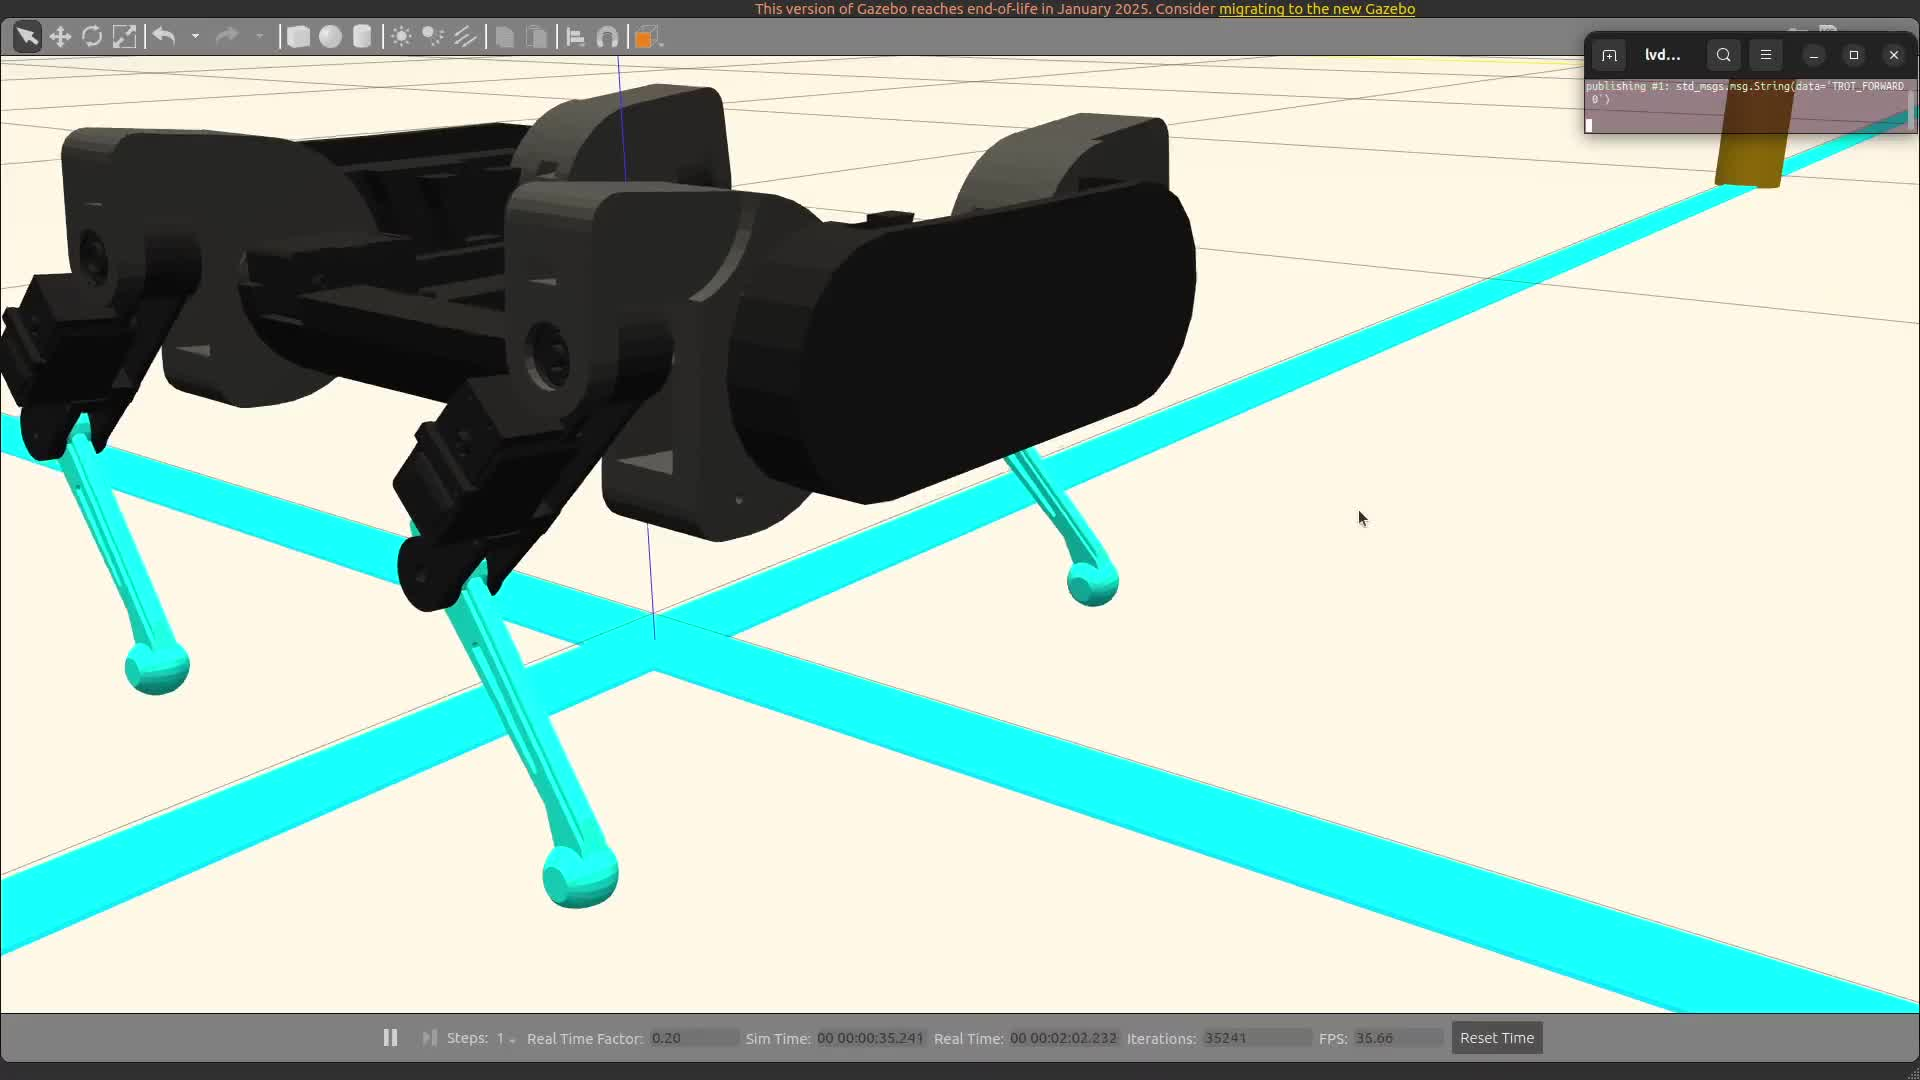
\includegraphics[width=\textwidth]{sim_trot_frames/frame_001.jpg}
        \caption{0.0s}
    \end{subfigure}
    \hfill
    \begin{subfigure}[b]{0.19\textwidth}
        \centering
        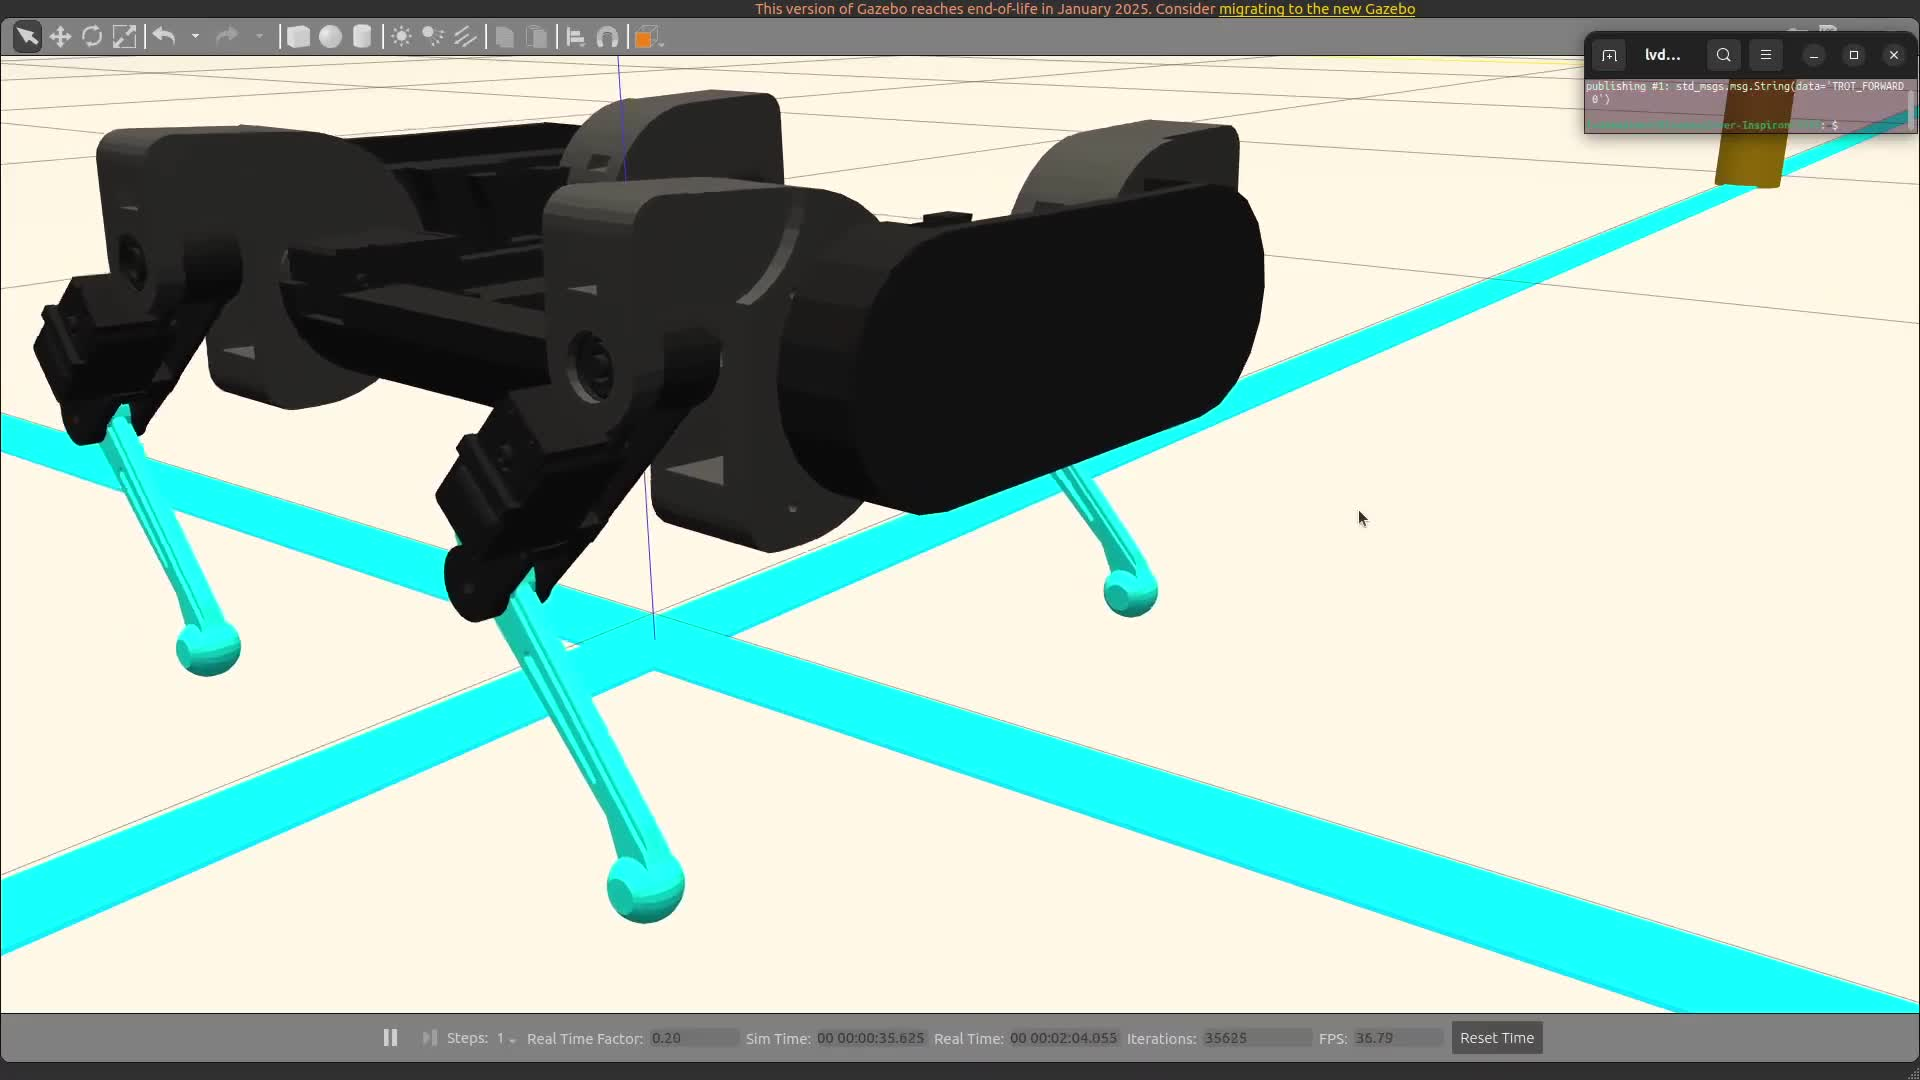
\includegraphics[width=\textwidth]{sim_trot_frames/frame_002.jpg}
        \caption{2.0s}
    \end{subfigure}
    \hfill
    \begin{subfigure}[b]{0.19\textwidth}
        \centering
        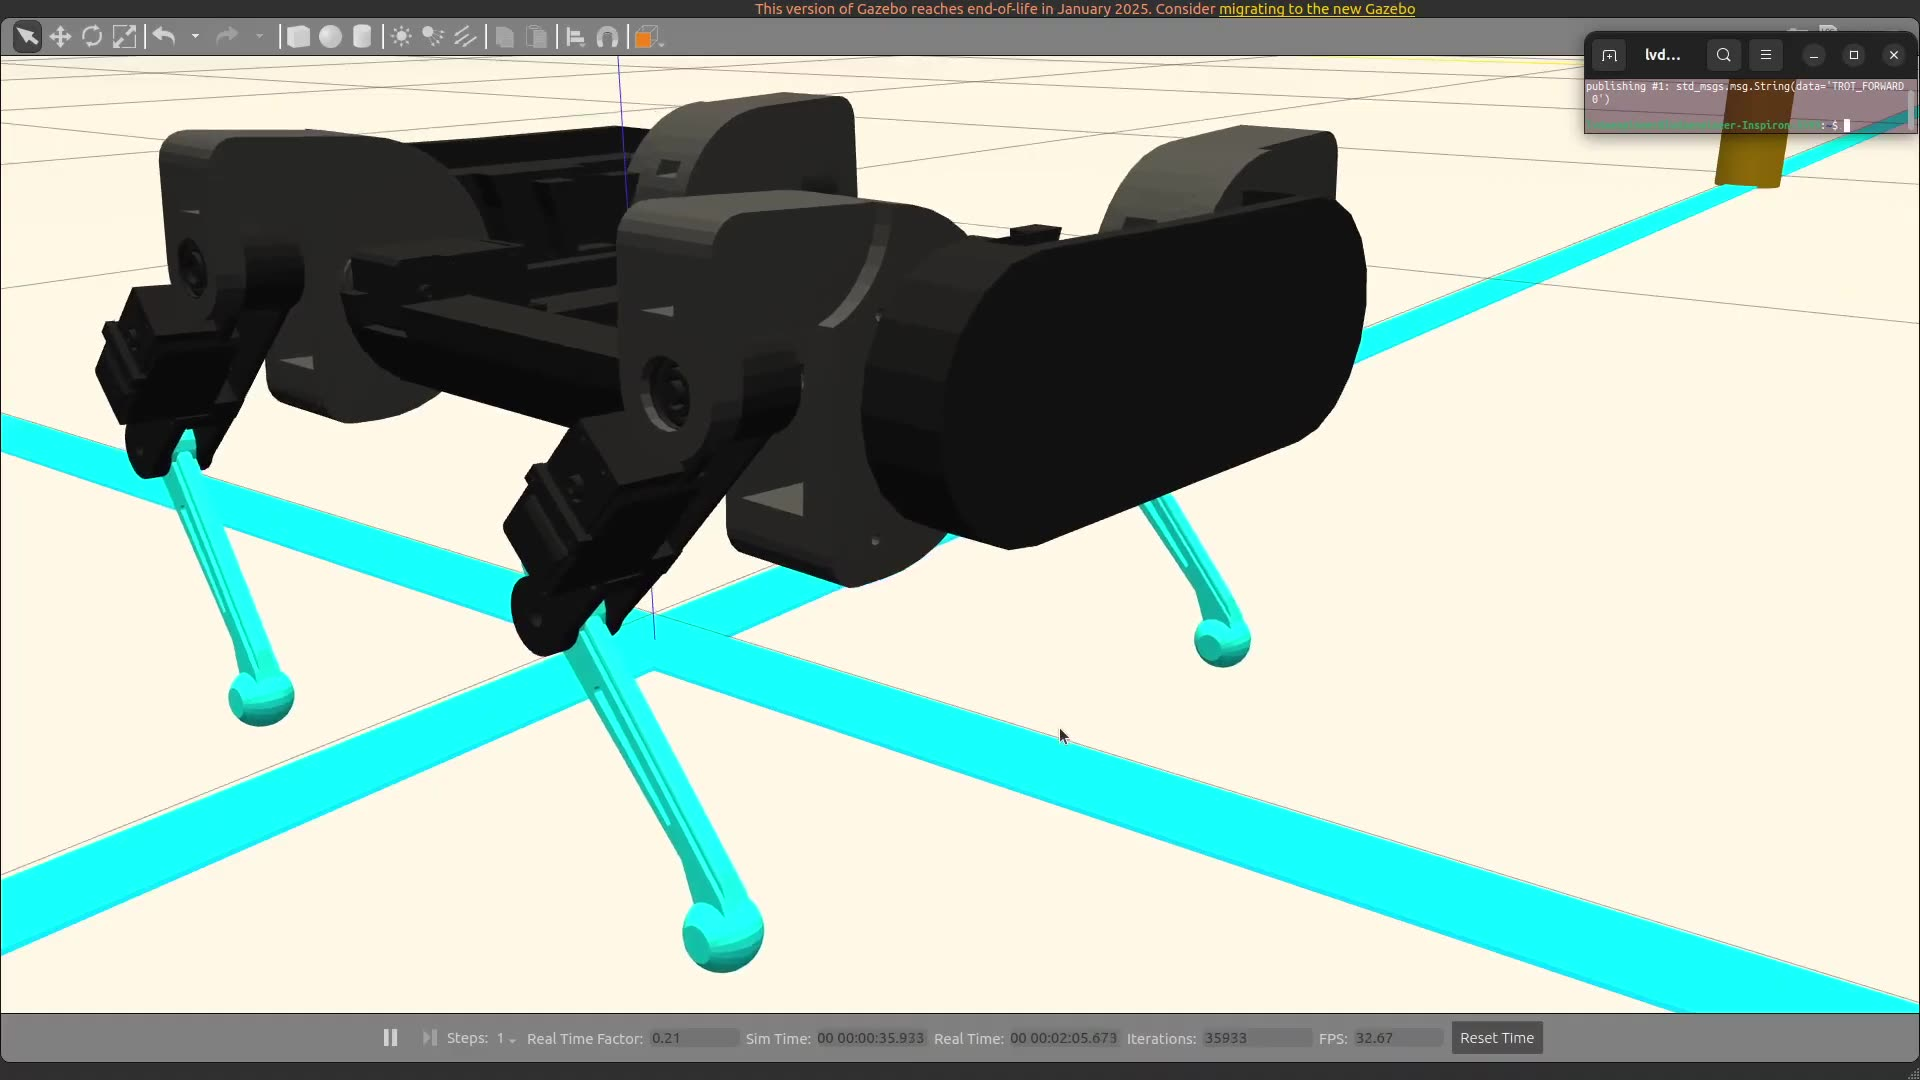
\includegraphics[width=\textwidth]{sim_trot_frames/frame_003.jpg}
        \caption{4.0s}
    \end{subfigure}
    \hfill
    \begin{subfigure}[b]{0.19\textwidth}
        \centering
        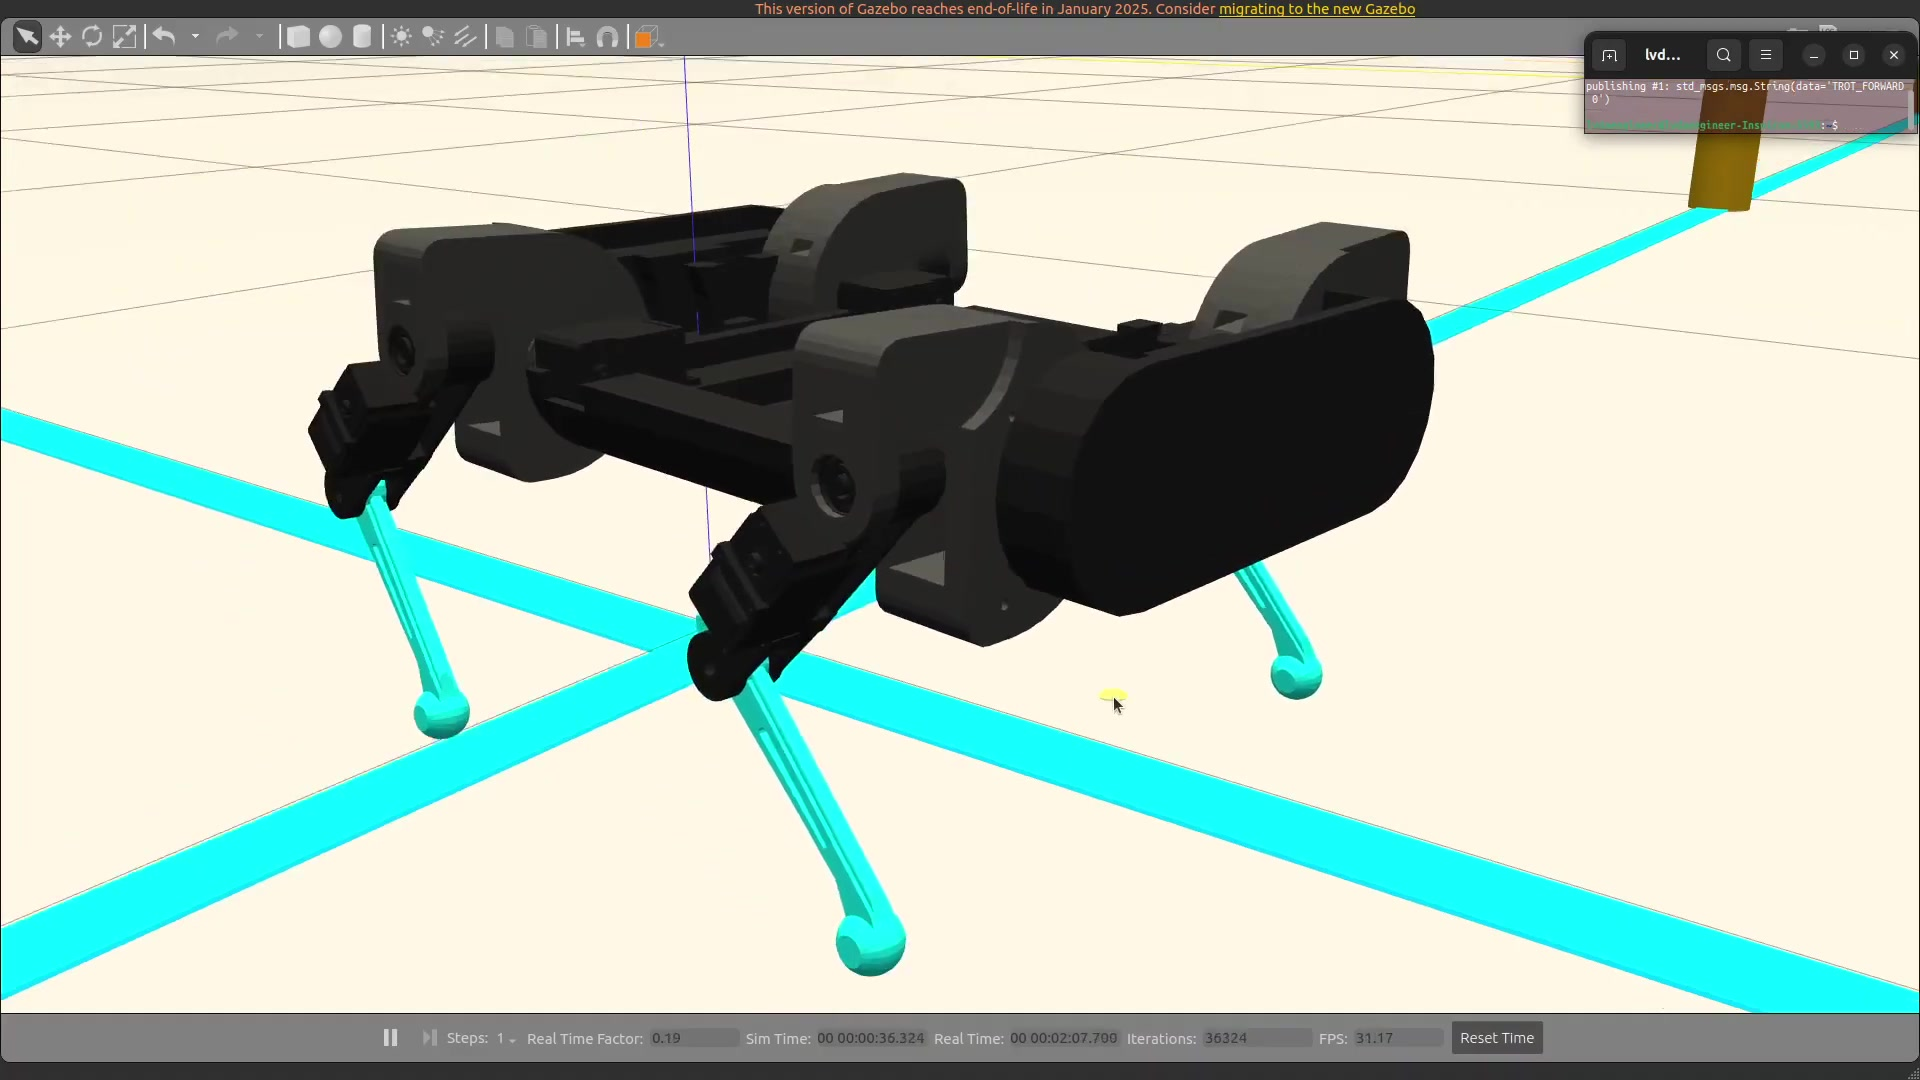
\includegraphics[width=\textwidth]{sim_trot_frames/frame_004.jpg}
        \caption{6.0s}
    \end{subfigure}
    \hfill
    \begin{subfigure}[b]{0.19\textwidth}
        \centering
        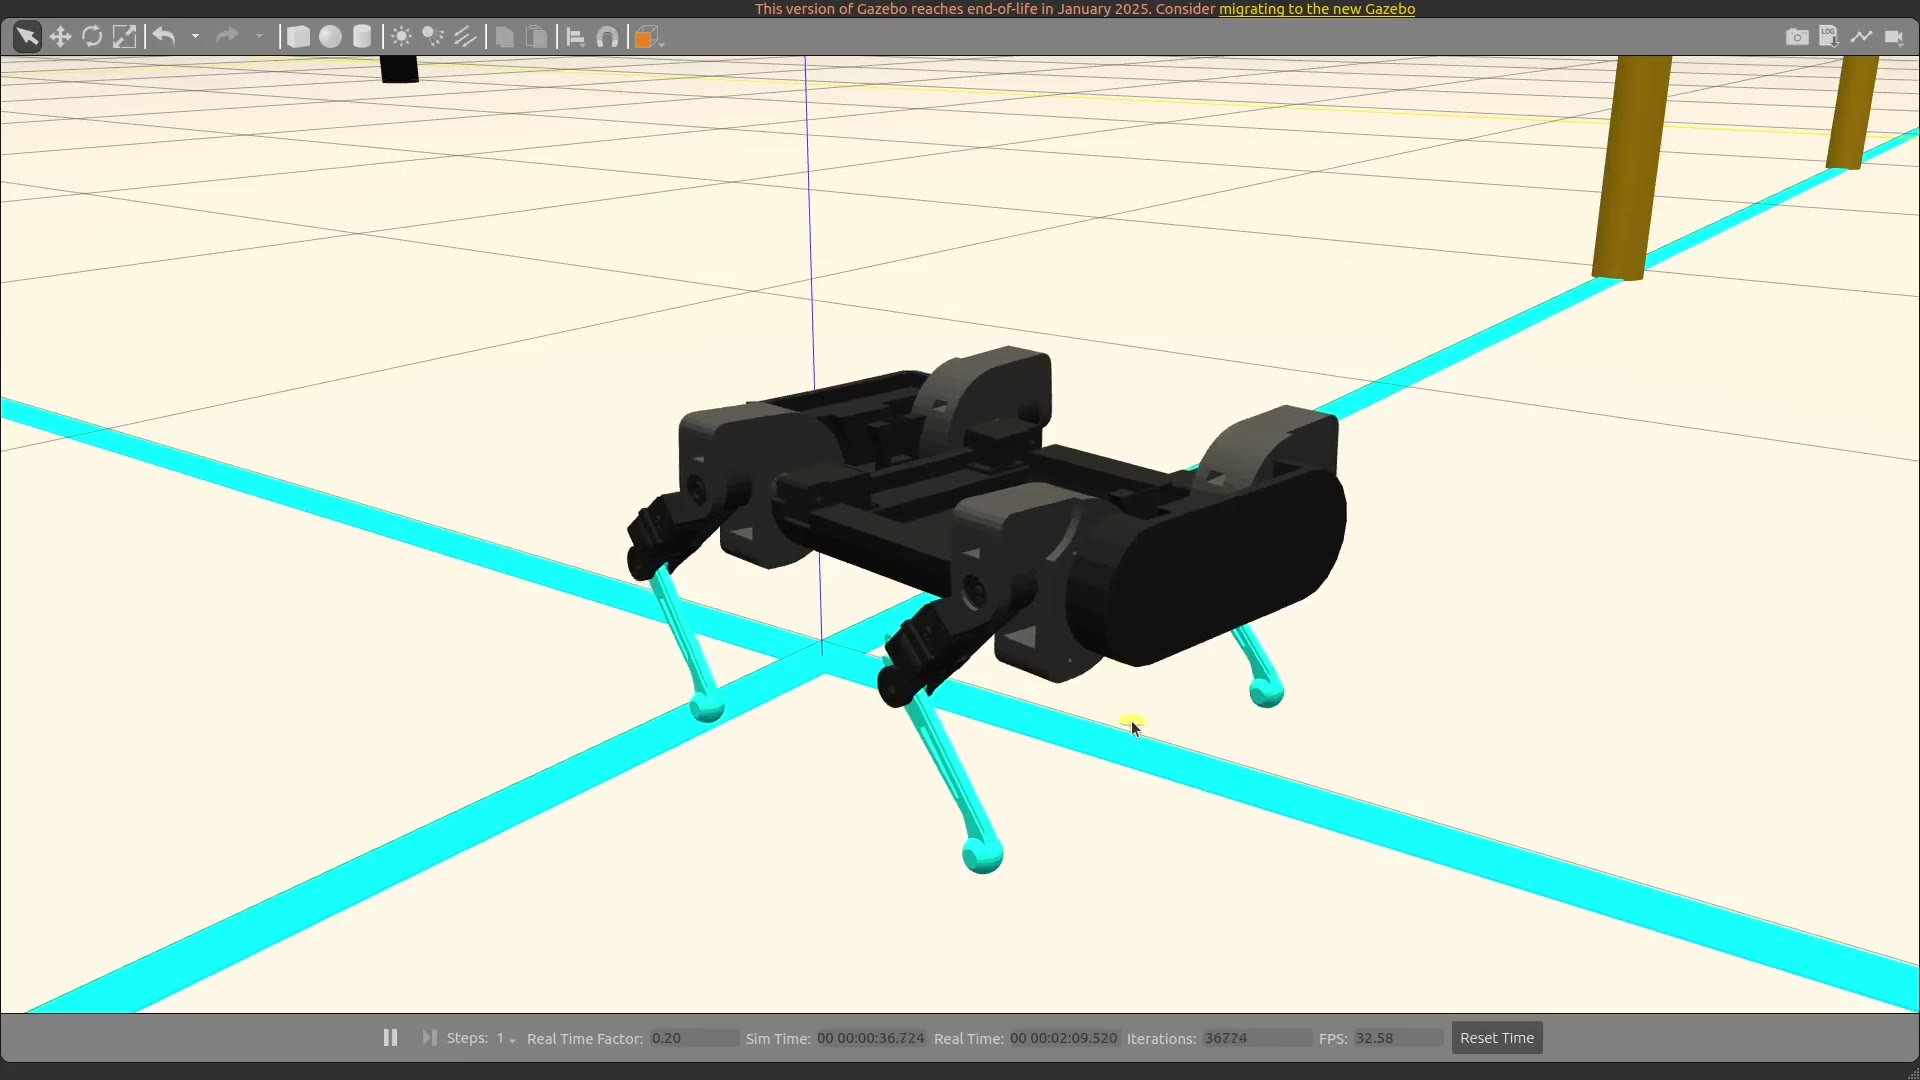
\includegraphics[width=\textwidth]{sim_trot_frames/frame_005.jpg}
        \caption{8.0s}
    \end{subfigure}
    
    \vspace{0.3cm} % Tạo khoảng trống giữa 2 hàng

    % ---- HÀNG 2: 5 ẢNH SAU ----
    \begin{subfigure}[b]{0.19\textwidth}
        \centering
        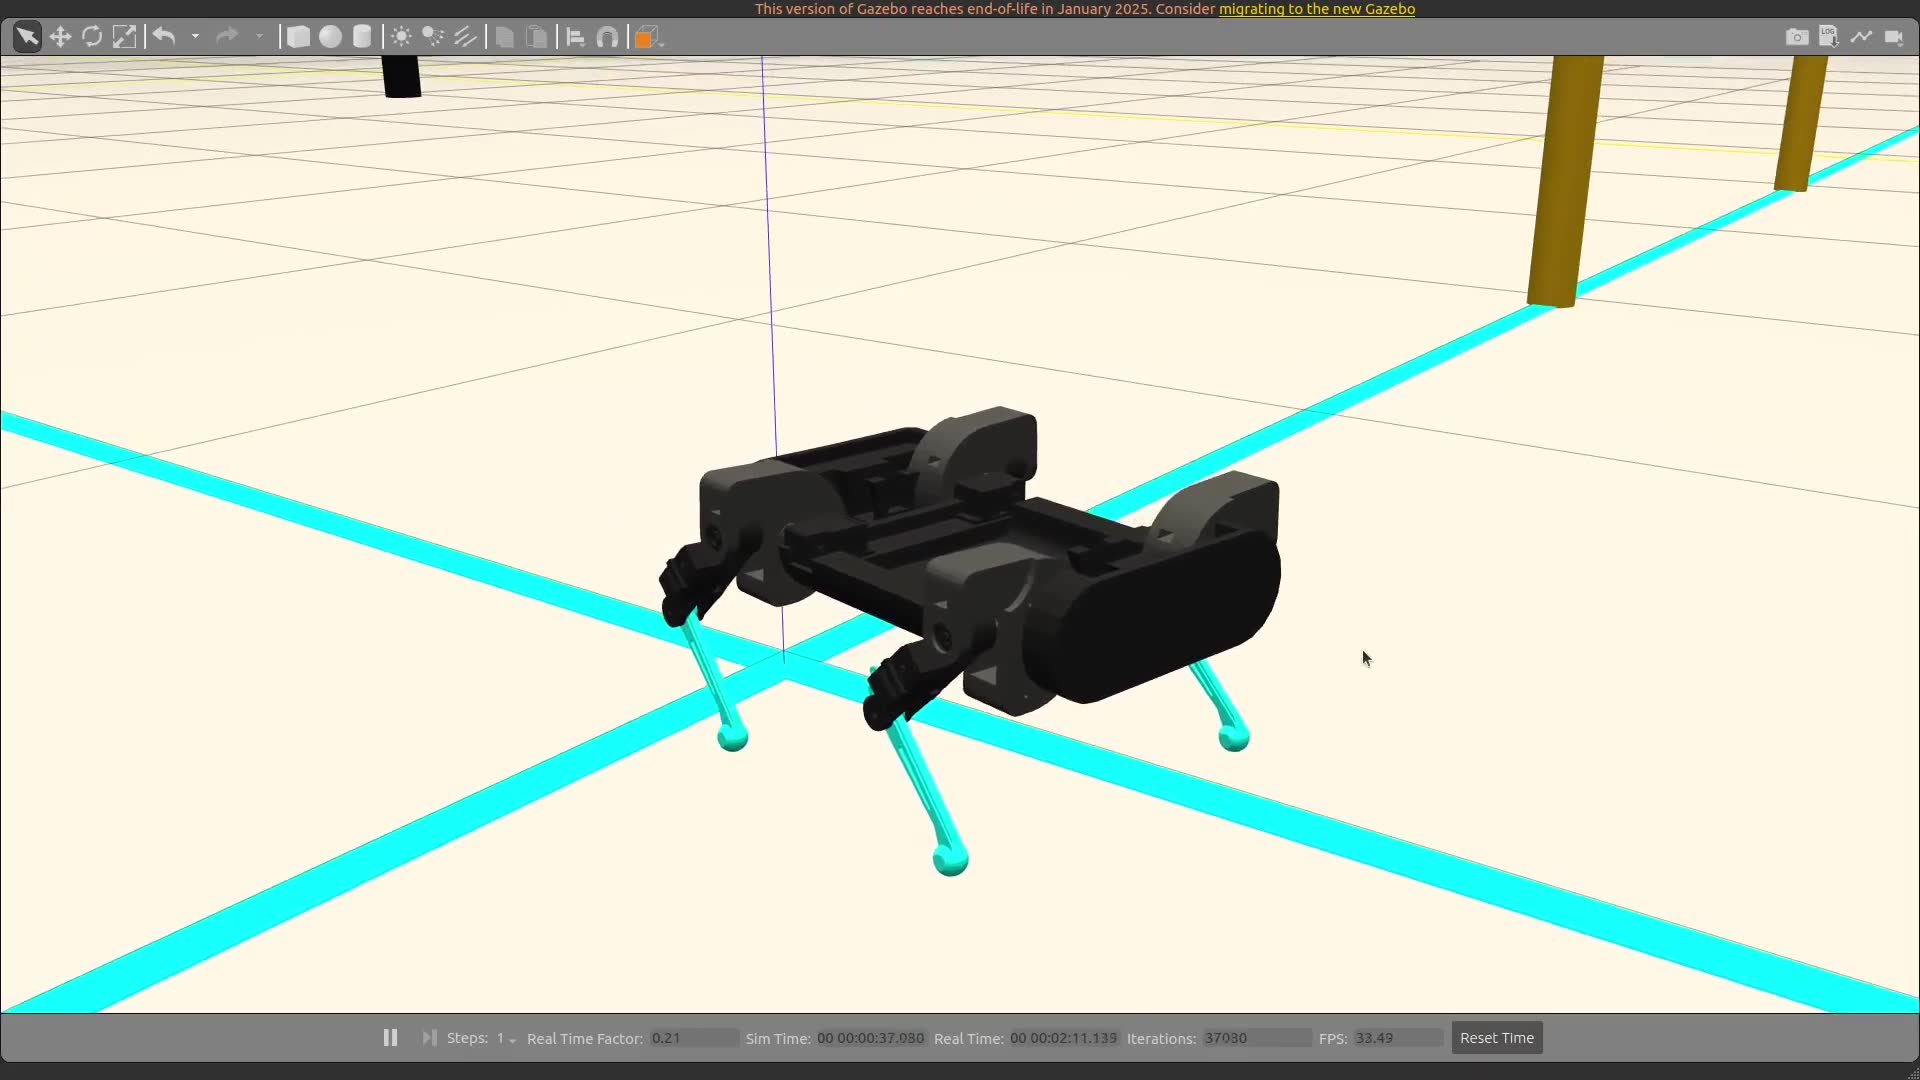
\includegraphics[width=\textwidth]{sim_trot_frames/frame_006.jpg}
        \caption{10.0s}
    \end{subfigure}
    \hfill
    \begin{subfigure}[b]{0.19\textwidth}
        \centering
        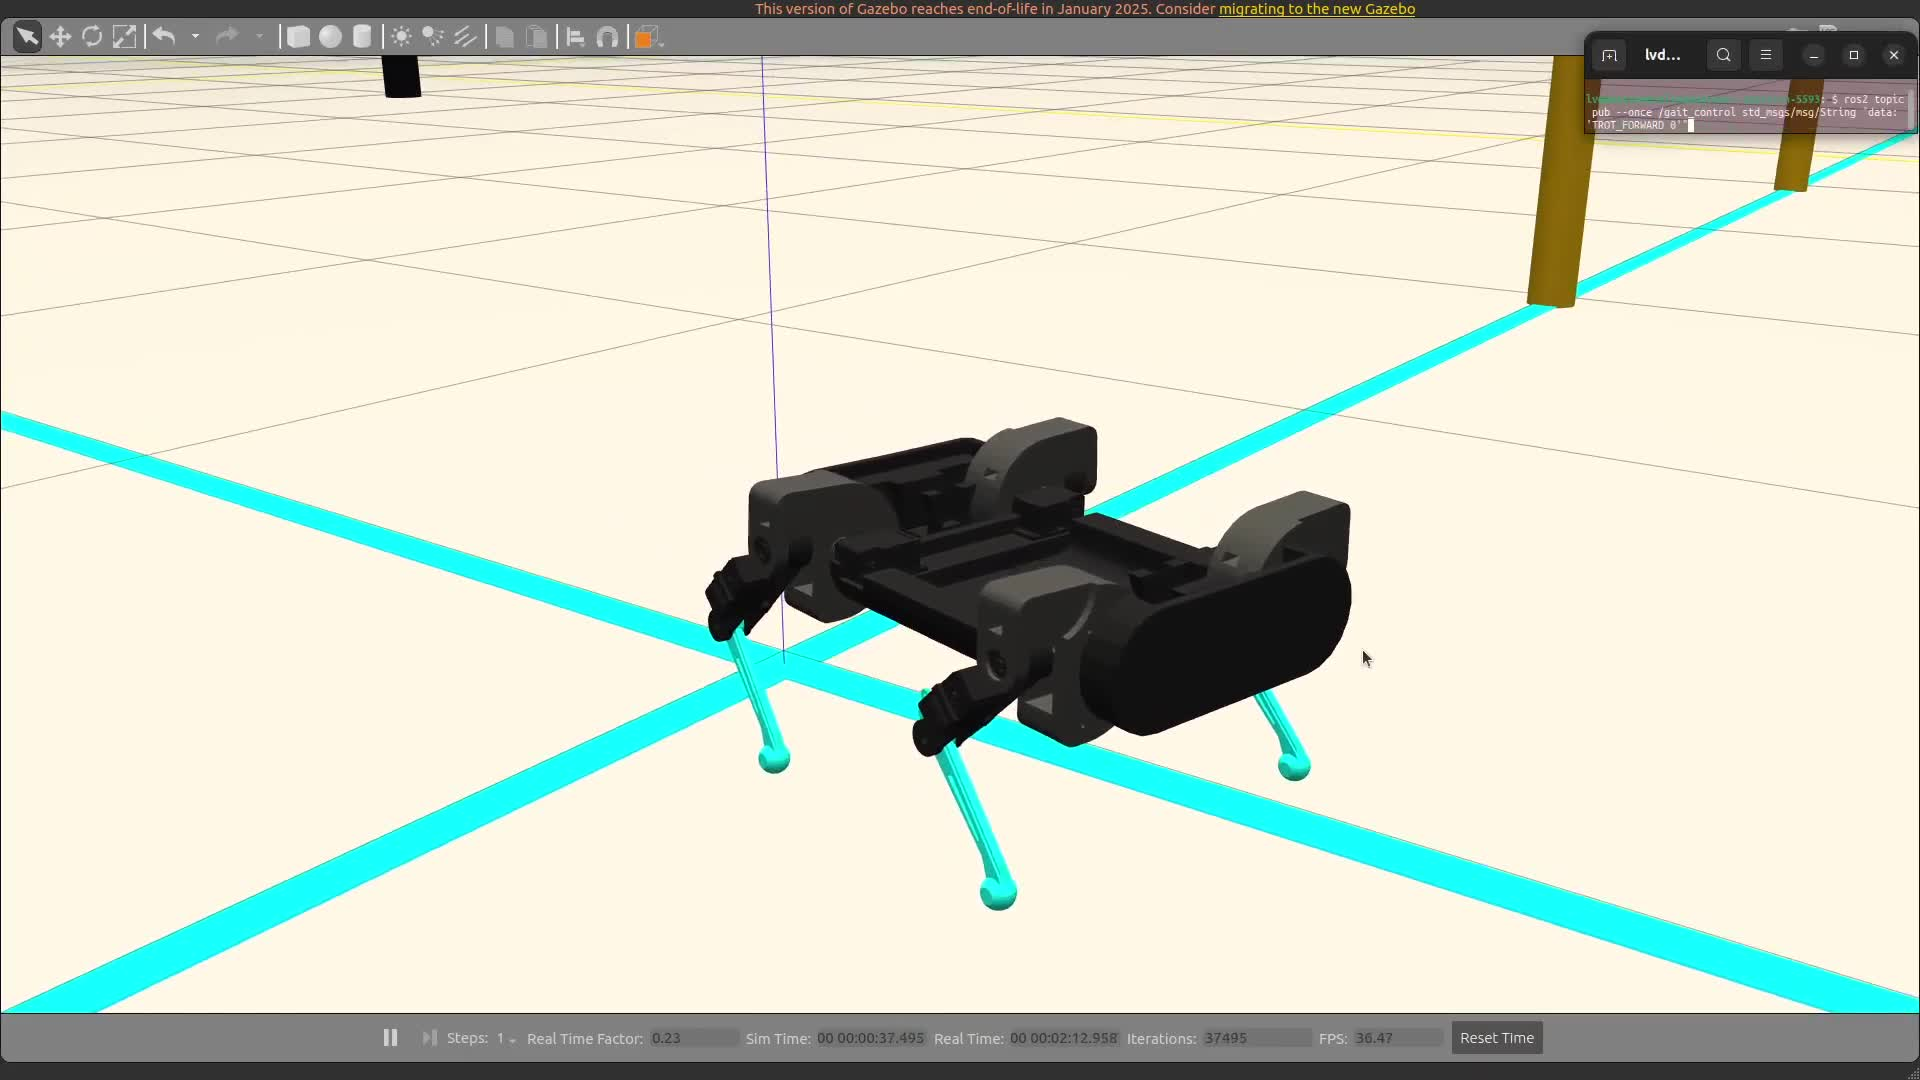
\includegraphics[width=\textwidth]{sim_trot_frames/frame_007.jpg}
        \caption{12.0s}
    \end{subfigure}
    \hfill
    \begin{subfigure}[b]{0.19\textwidth}
        \centering
        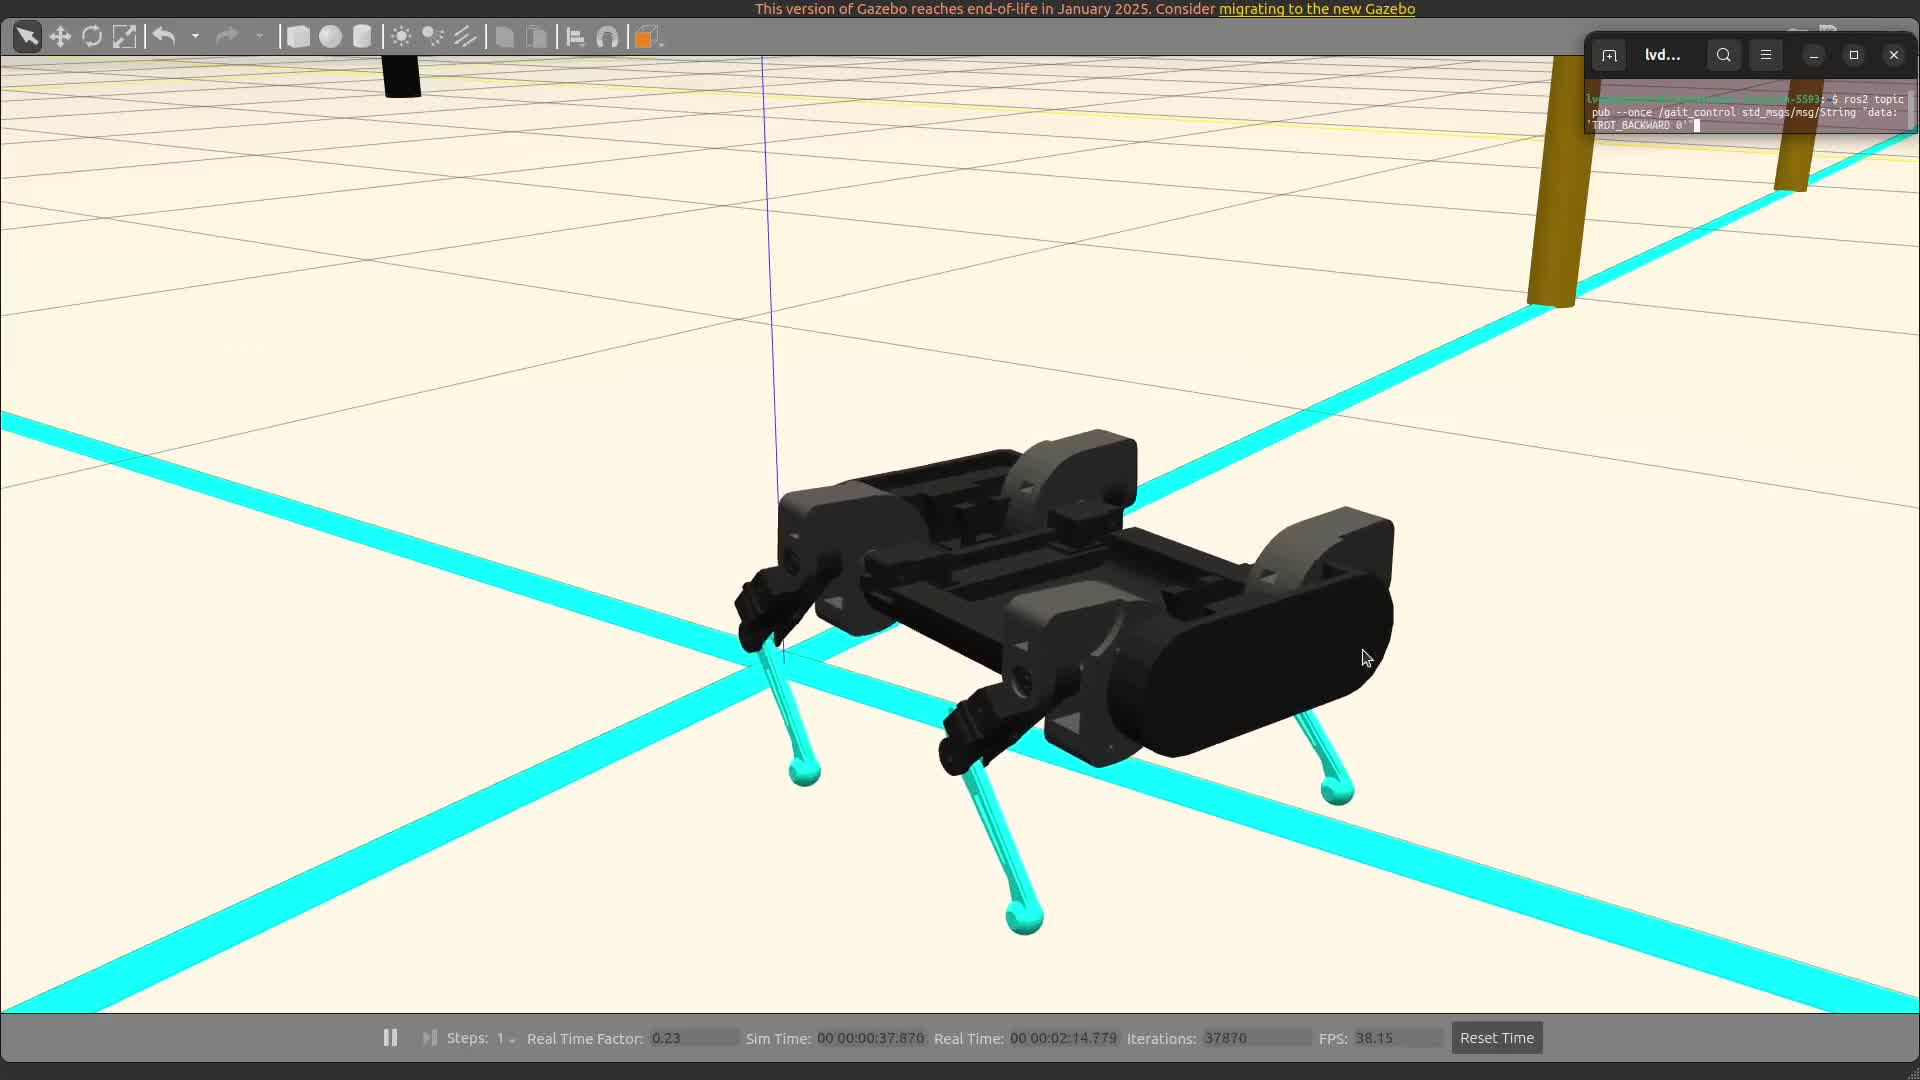
\includegraphics[width=\textwidth]{sim_trot_frames/frame_008.jpg}
        \caption{14.0s}
    \end{subfigure}
    \hfill
    \begin{subfigure}[b]{0.19\textwidth}
        \centering
        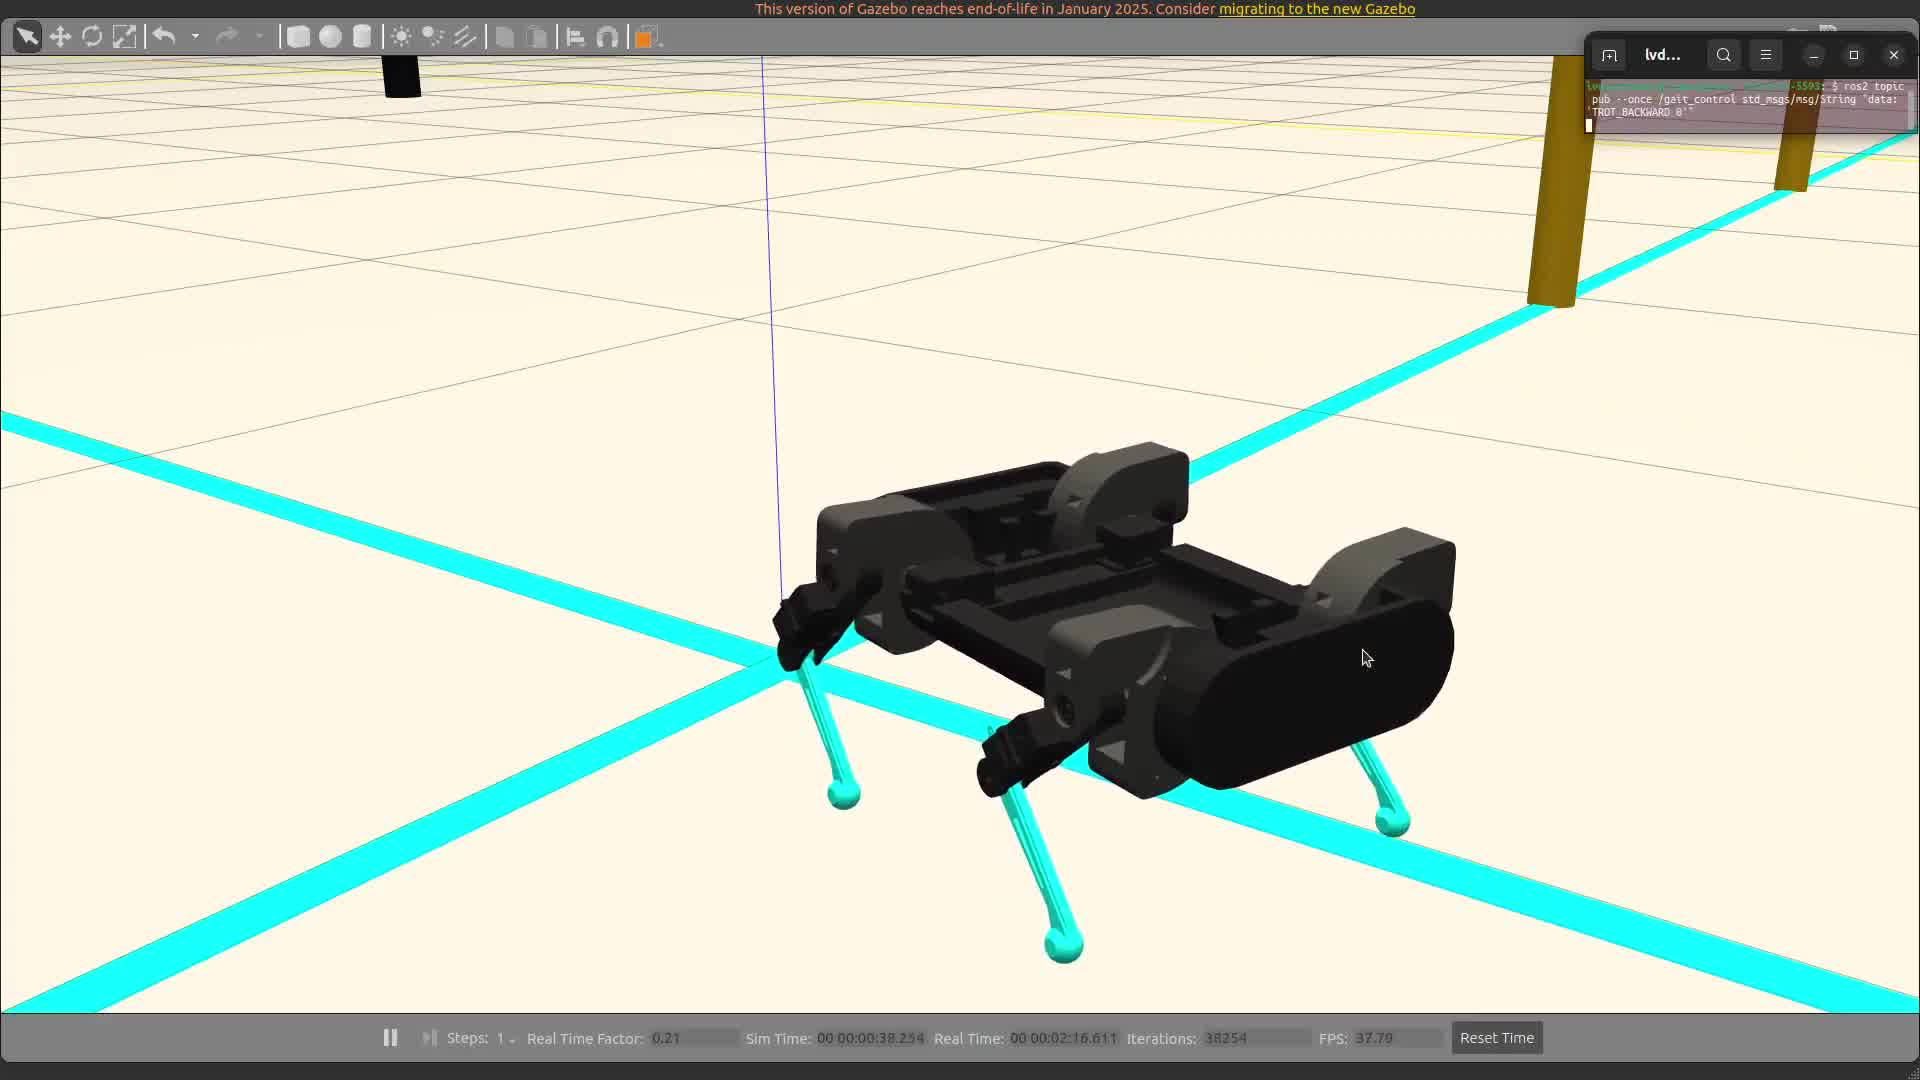
\includegraphics[width=\textwidth]{sim_trot_frames/frame_009.jpg}
        \caption{16.0s}
    \end{subfigure}
    \hfill
    \begin{subfigure}[b]{0.19\textwidth}
        \centering
        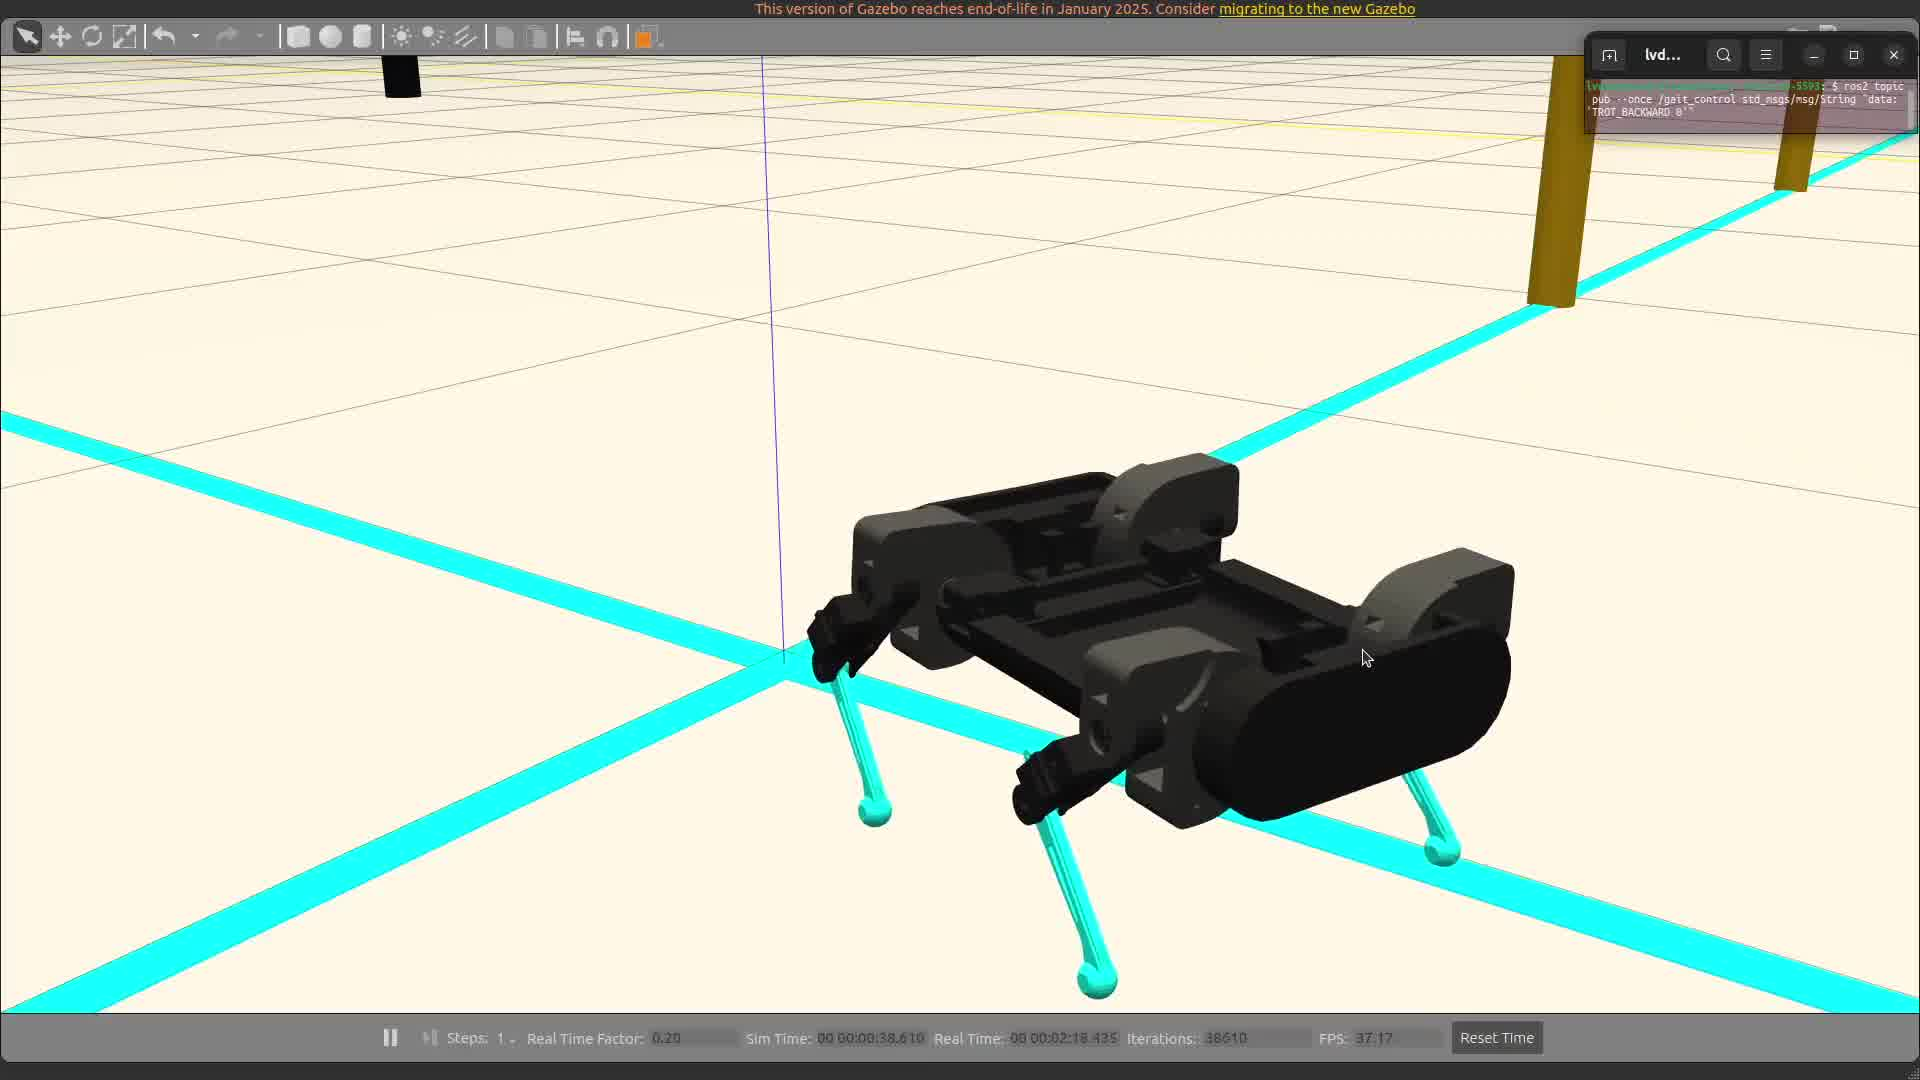
\includegraphics[width=\textwidth]{sim_trot_frames/frame_010.jpg}
        \caption{18.0s}
    \end{subfigure}

   \caption{Chuỗi hình ảnh mô phỏng quá trình robot thực hiện dáng đi Trot liên tục}
    \label{fig:timelapse_trot_gazebo}
\end{figure}

\section{Phân tích quỹ đạo bàn chân}

\subsection{Quỹ đạo trong mặt phẳng 2D}
\begin{figure}[H]
    \centering
    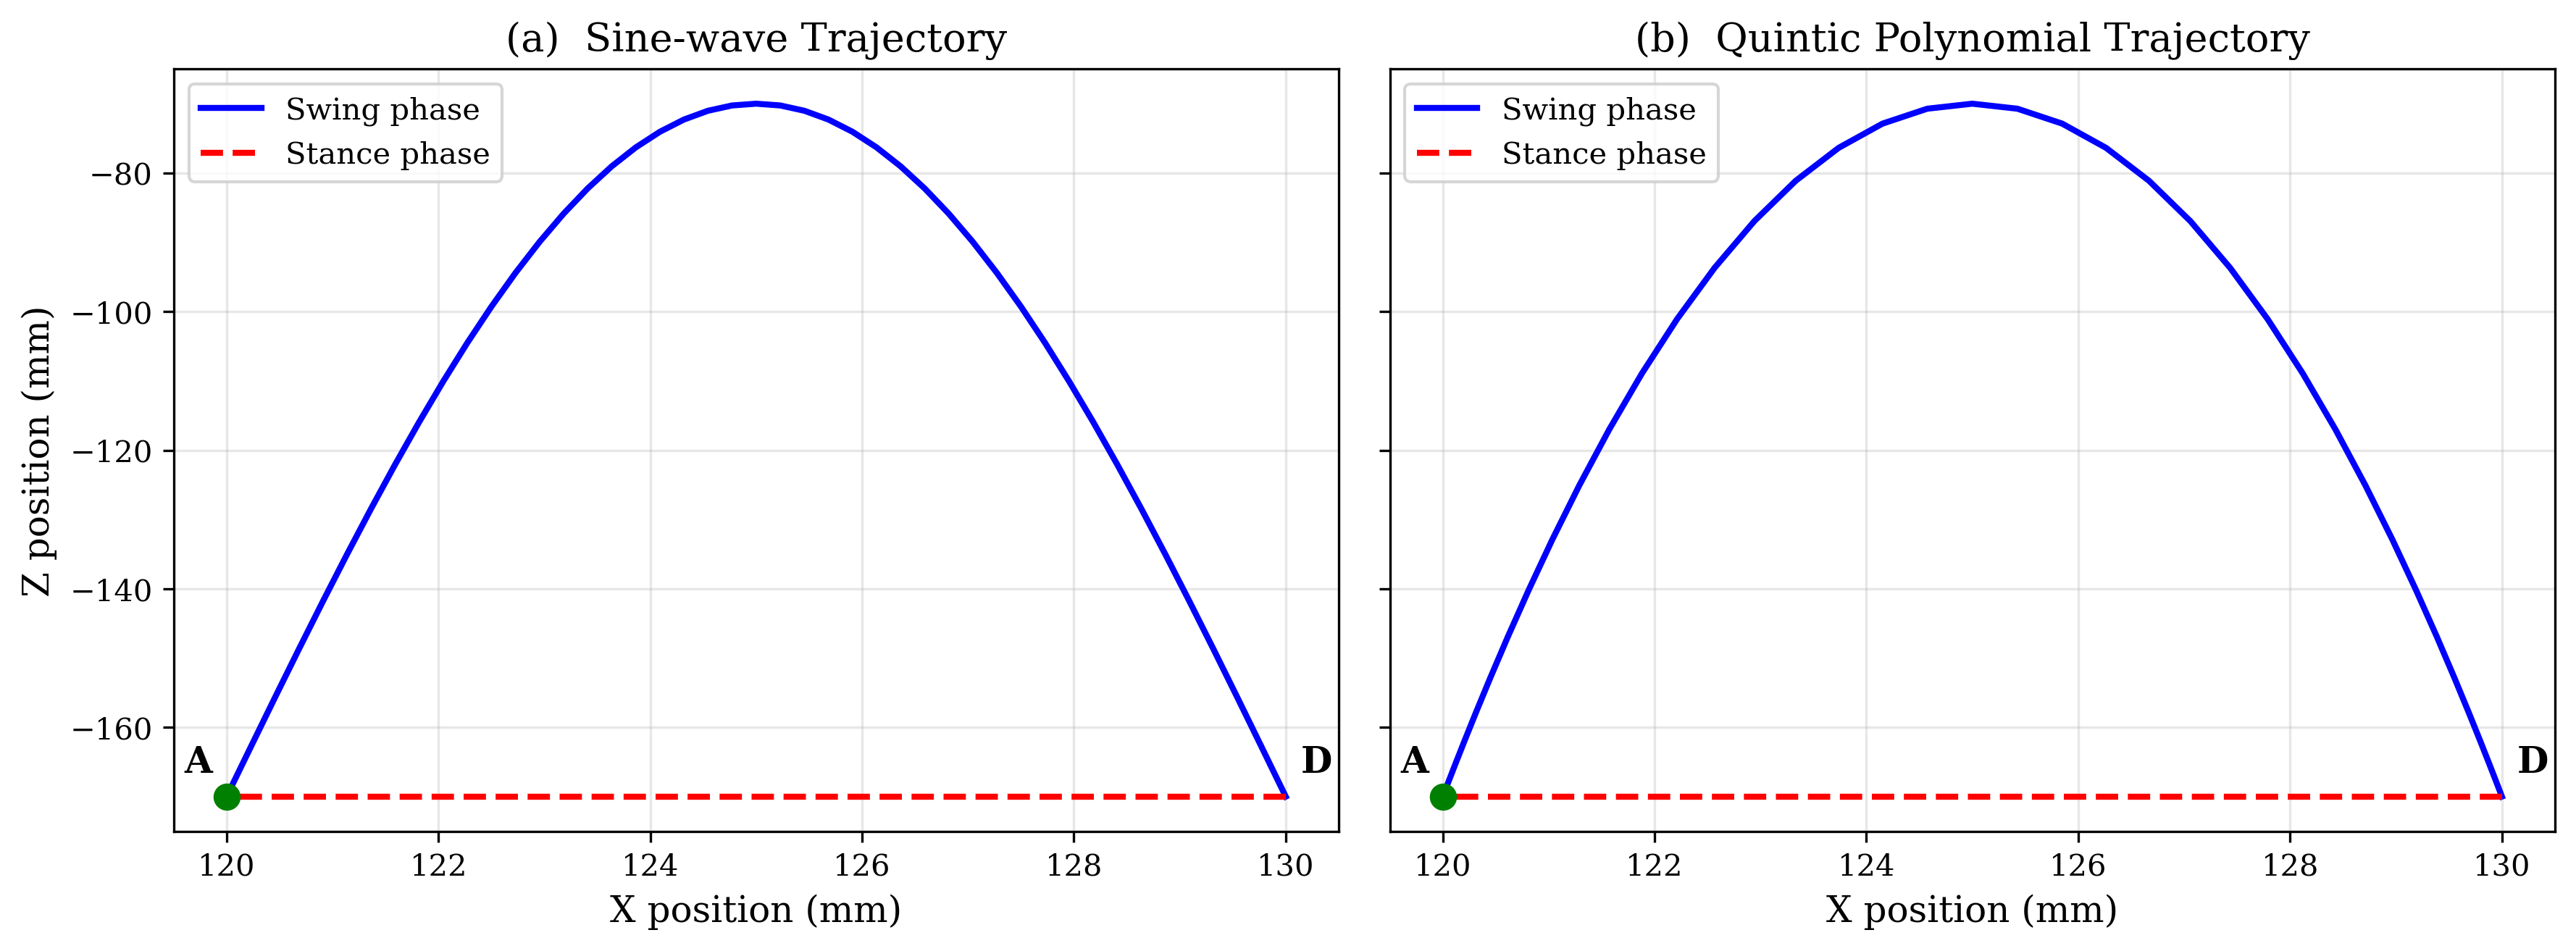
\includegraphics[width=0.6\textwidth]{Simulation/fig1_foot_trajectory_2d.png}
    \caption{Quỹ đạo bàn chân trong không gian 2D}
    \label{Simulation/fig1}
\end{figure}
Hình \ref{Simulation/fig1} trình bày quỹ đạo bàn chân trong mặt phẳng XZ (mặt phẳng sagittal), so sánh hai phương pháp lập kế hoạch: sóng sin (sine-wave) và đa thức bậc 5 (quintic polynomial).

Quỹ đạo bàn chân có dạng hình chữ D, bao gồm hai pha: pha swing (nâng chân) trong đó bàn chân di chuyển theo đường cong từ điểm A đến điểm D với độ nâng $h = 40$ mm so với mặt đất, và pha stance (chạm đất) trong đó bàn chân trượt ngược trên mặt đất tạo lực đẩy cho robot.

Phương pháp sóng sin sử dụng hàm sin để tạo biên dạng nâng chân. Ưu điểm là đơn giản trong triển khai, tuy nhiên không kiểm soát được vận tốc và gia tốc tại các điểm chuyển pha. Phương pháp đa thức bậc 5 sử dụng hàm $s(\tau) = 10\tau^3 - 15\tau^4 + 6\tau^5$ với $\tau \in [0, 1]$, đảm bảo các điều kiện biên: $s(0) = 0$, $s(1) = 1$, $s'(0) = s'(1) = 0$, $s''(0) = s''(1) = 0$. Nhờ đó, quỹ đạo có tính liên tục bậc hai (C$^2$), giảm thiểu rung lắc cơ khí tại các điểm chuyển pha.

\subsection{Quỹ đạo trong không gian 3D}
\begin{figure}[H]
    \centering
    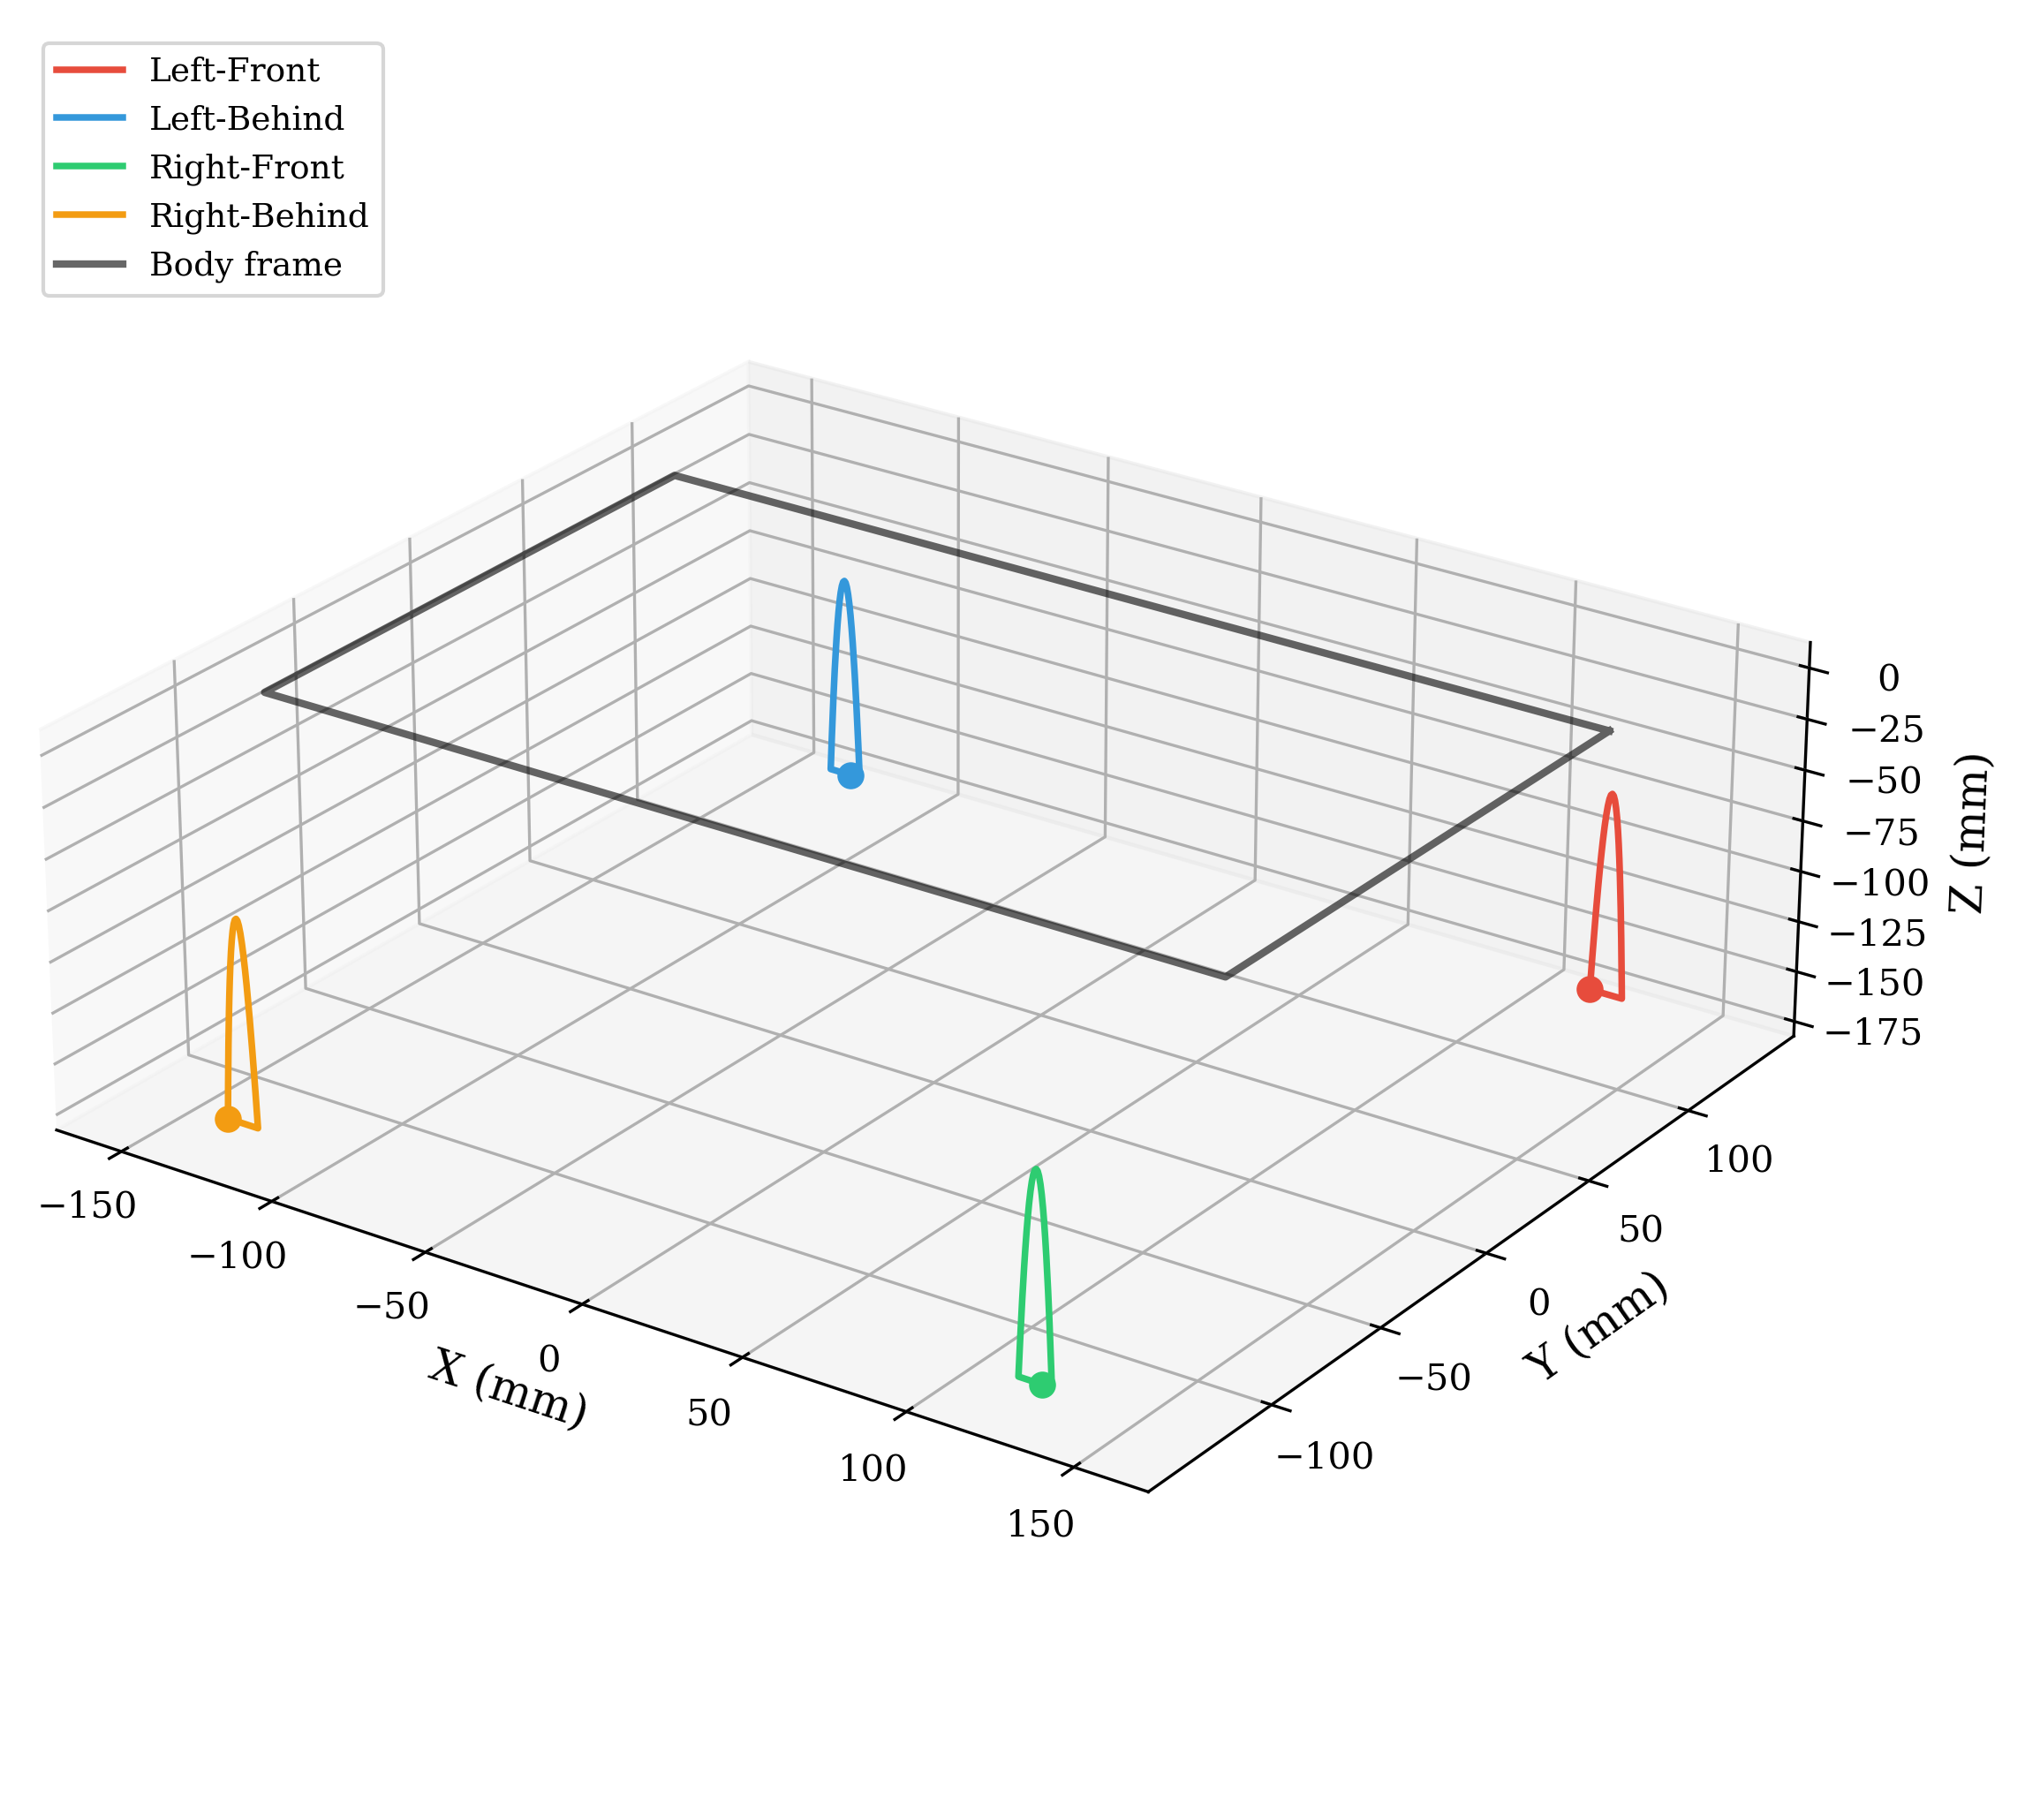
\includegraphics[width=0.6\textwidth]{Simulation/fig2_foot_trajectory_3d.png}
    \caption{Quỹ đạo bàn chân trong không gian 3D}
    \label{Simulation/fig2}
\end{figure}
Hình \ref{Simulation/fig2} hiển thị quỹ đạo 3D của cả bốn chân trong hệ tọa độ thân robot (body frame), với kích thước thân $L \times W = 120 \times 90$ mm. Bốn quỹ đạo hình chữ D được phân bố tại bốn góc của khung thân, mỗi chân có offset pha tương ứng với dáng đi Trot. Dáng đi này có đặc điểm hai chân chéo nhau cùng thực hiện pha swing (LF+RB và LB+RF luân phiên), đảm bảo tại mọi thời điểm luôn có ít nhất hai chân chạm đất.

\subsection{Biên dạng vận tốc và gia tốc}
\begin{figure}[H]
    \centering
    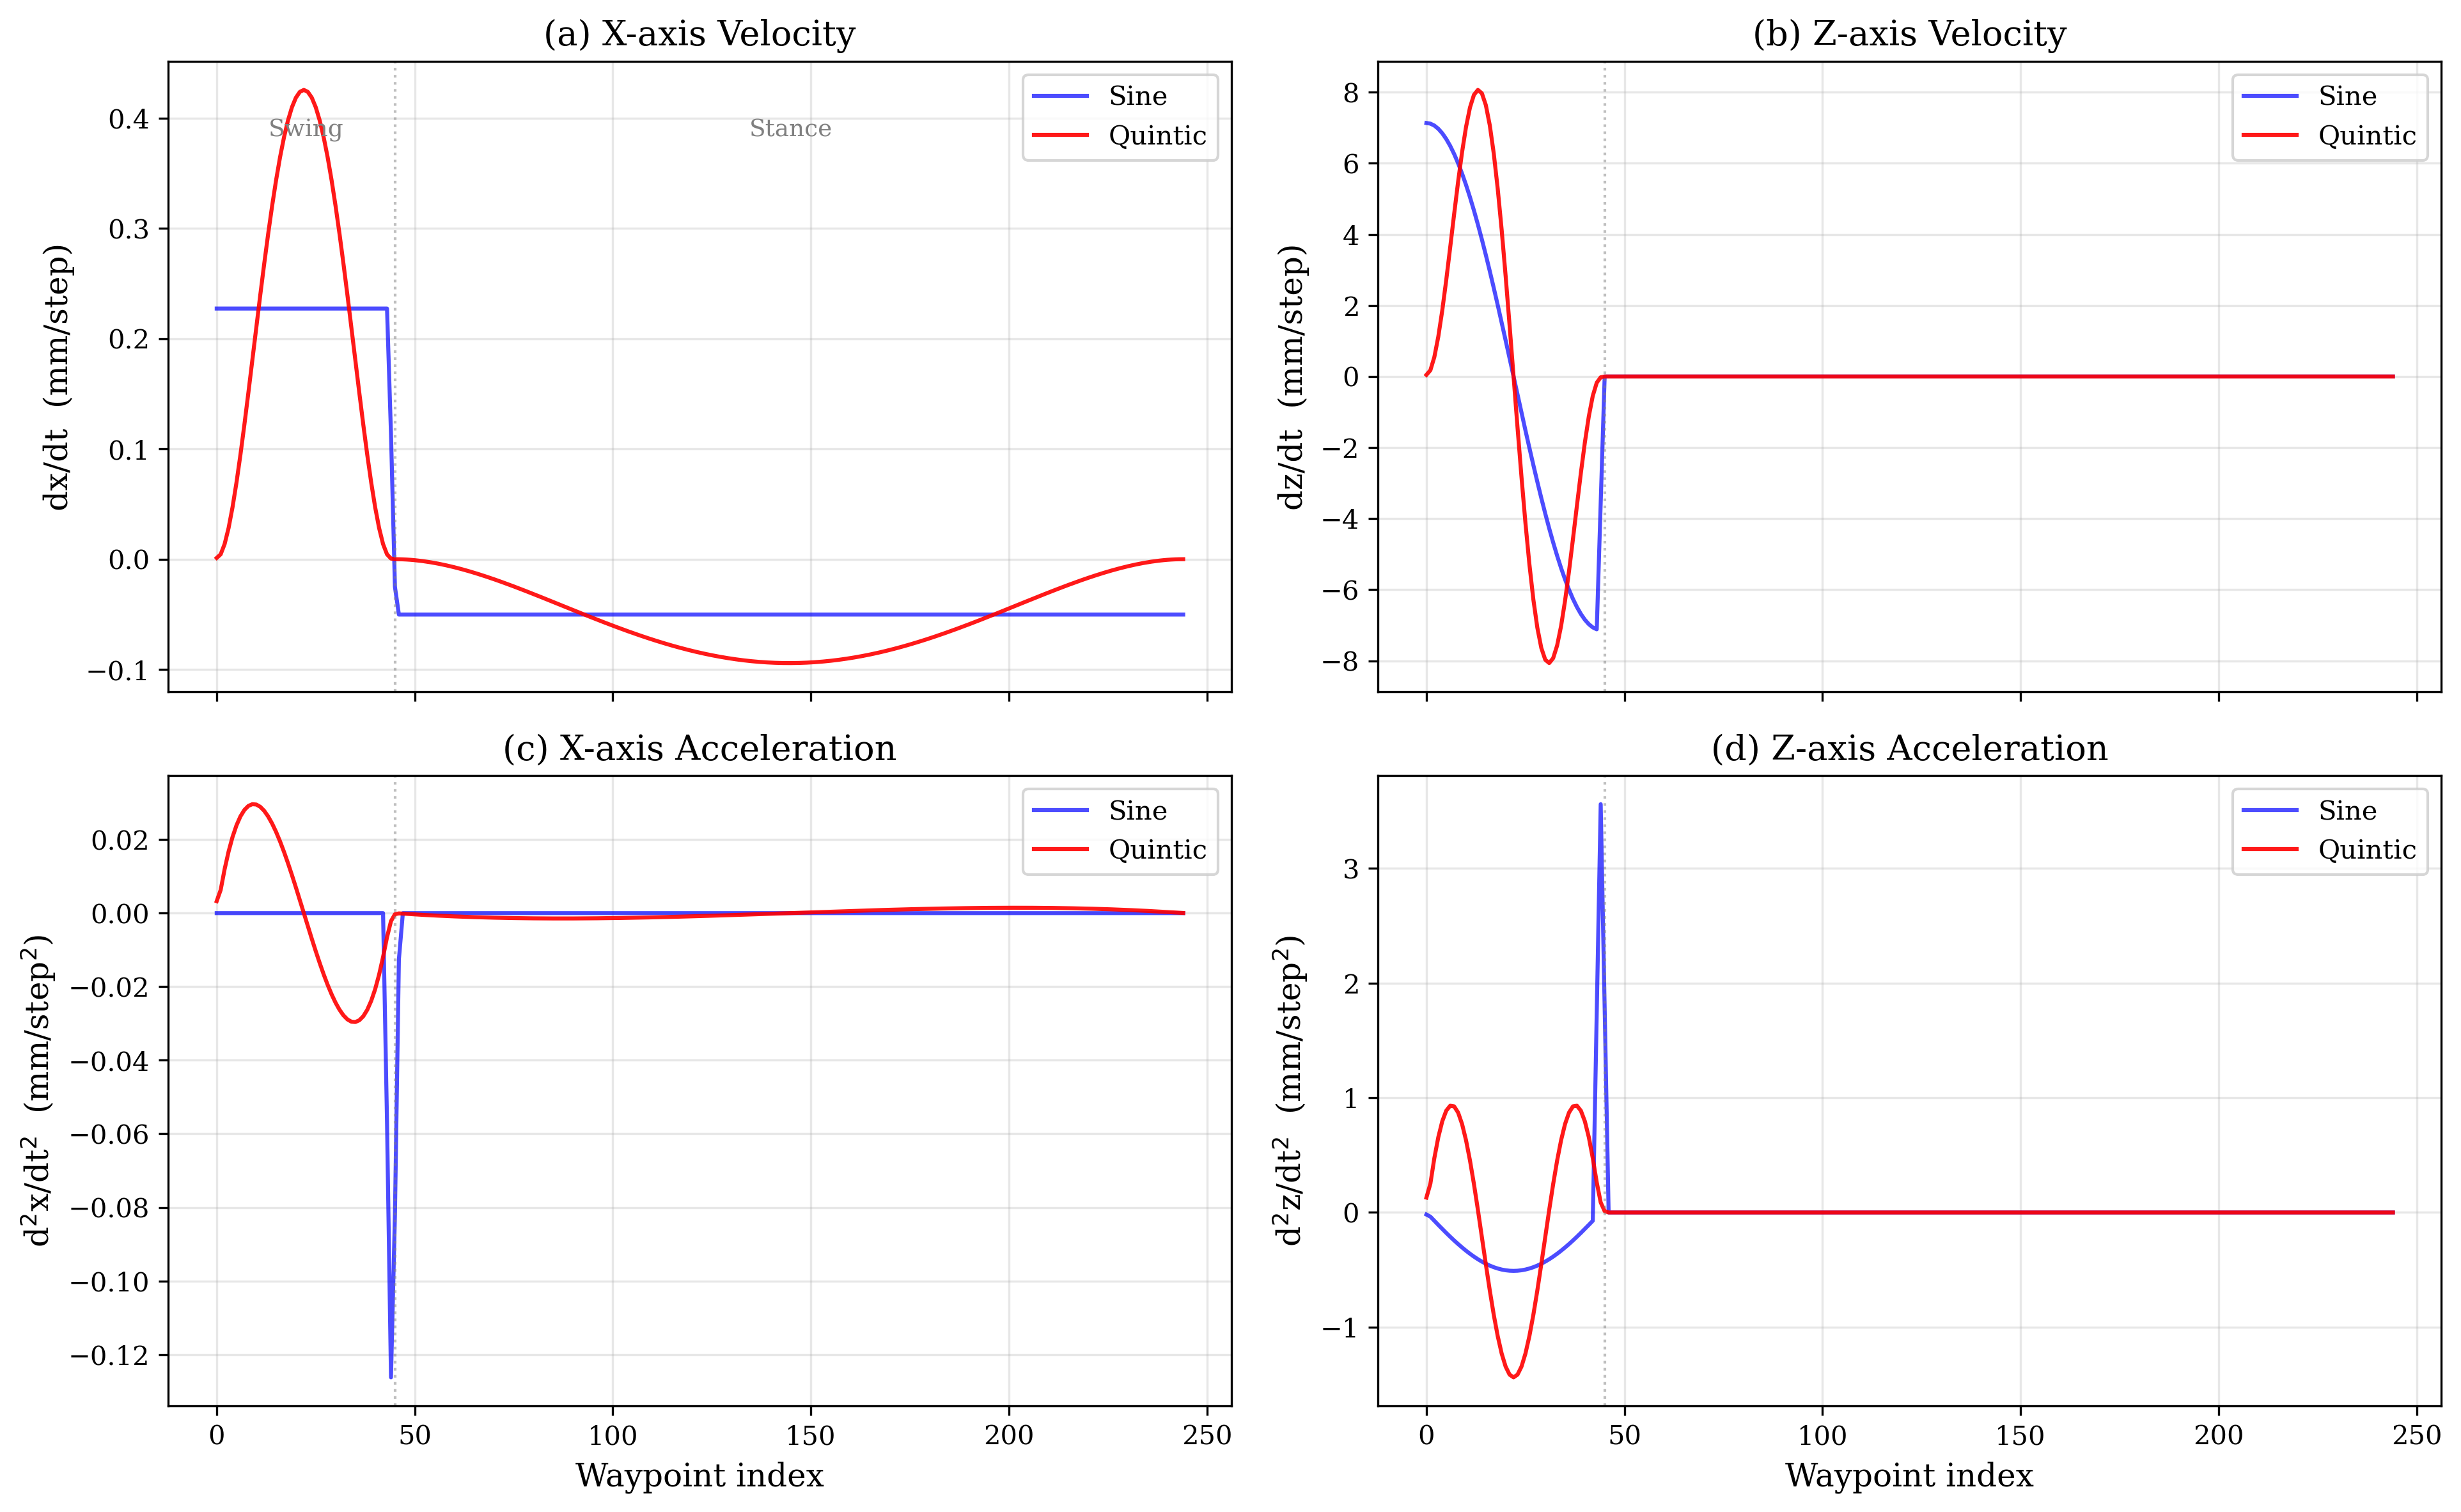
\includegraphics[width=0.6\textwidth]{Simulation/fig3_velocity_acceleration.png}
    \caption{Biên dạng vận tốc và gia tốc}
    \label{Simulation/fig3}
\end{figure}
Hình \ref{Simulation/fig3} so sánh biên dạng vận tốc và gia tốc của bàn chân theo hai trục X và Z giữa hai phương pháp, gồm bốn subplot:

Subplot (a) và (b) thể hiện vận tốc theo trục X ($dx/dt$) và trục Z ($dz/dt$). Kết quả cho thấy phương pháp đa thức bậc 5 có vận tốc bằng 0 tại cả hai đầu pha swing, trong khi phương pháp sóng sin có bước nhảy vận tốc tại ranh giới chuyển pha swing-stance.

Subplot (c) và (d) thể hiện gia tốc theo trục X ($d^2x/dt^2$) và trục Z ($d^2z/dt^2$). Sự khác biệt rõ rệt nhất ở biên dạng gia tốc: phương pháp sóng sin tạo các đỉnh gia tốc đột ngột (gián đoạn), trong khi đa thức bậc 5 cho biên dạng gia tốc liên tục. Kết quả này chứng minh rằng phương pháp đa thức bậc 5 ưu việt hơn về mặt mượt mà động học, giảm thiểu rung lắc và lực va đập tại các khớp.

\subsection{Phân tích biến thiên quỹ đạo theo các trục tọa độ}

\begin{figure}[H]
    \centering
    
\includegraphics[width=0.85\textwidth]{fig26- Fifth degree profiling curve.png}
    \caption{Sự biến thiên vị trí, vận tốc và gia tốc của 3 trục X, Y, Z trong chu kỳ bước đầy đủ}
    \label{fig:xyz_trajectory_full}
\end{figure}

Hình \ref{fig:xyz_trajectory_full} minh họa chi tiết sự biến thiên của ba trục tọa độ không gian (X, Y, Z) đối với vị trí, vận tốc và gia tốc trong một chu kỳ bước hoàn chỉnh của robot. Dựa trên đồ thị, có thể thấy rõ các pha của chuyển động: pha vung chân (swing phase) diễn ra từ $\tau = 0$ đến $\tau = 0.4$, trong đó trục Z nhấc lên thành hình vòm cong; pha chống chân (stance phase) kéo dài từ $\tau = 0.4$ đến $\tau = 1.0$, trong đó trục Z duy trì hằng số và trục X trượt ngược lại tạo lực đẩy tiến về phía trước. Đặc biệt, nhờ việc ứng dụng hàm nội suy chuẩn hóa bậc 5 (được phân tích ở Chương 4) làm hệ số nội suy cho cả 3 trục, biên dạng vận tốc và gia tốc của X, Y, Z đều hoàn toàn mượt mà, không xuất hiện điểm gãy khúc hay nhảy vọt gia tốc. Điều này một lần nữa khẳng định hiệu quả của việc đưa lý thuyết hàm cơ sở vào triển khai quỹ đạo thực tế.

\section{Phân tích góc khớp và mô-men xoắn}

\subsection{Biến thiên góc khớp}
\begin{figure}[H]
    \centering
    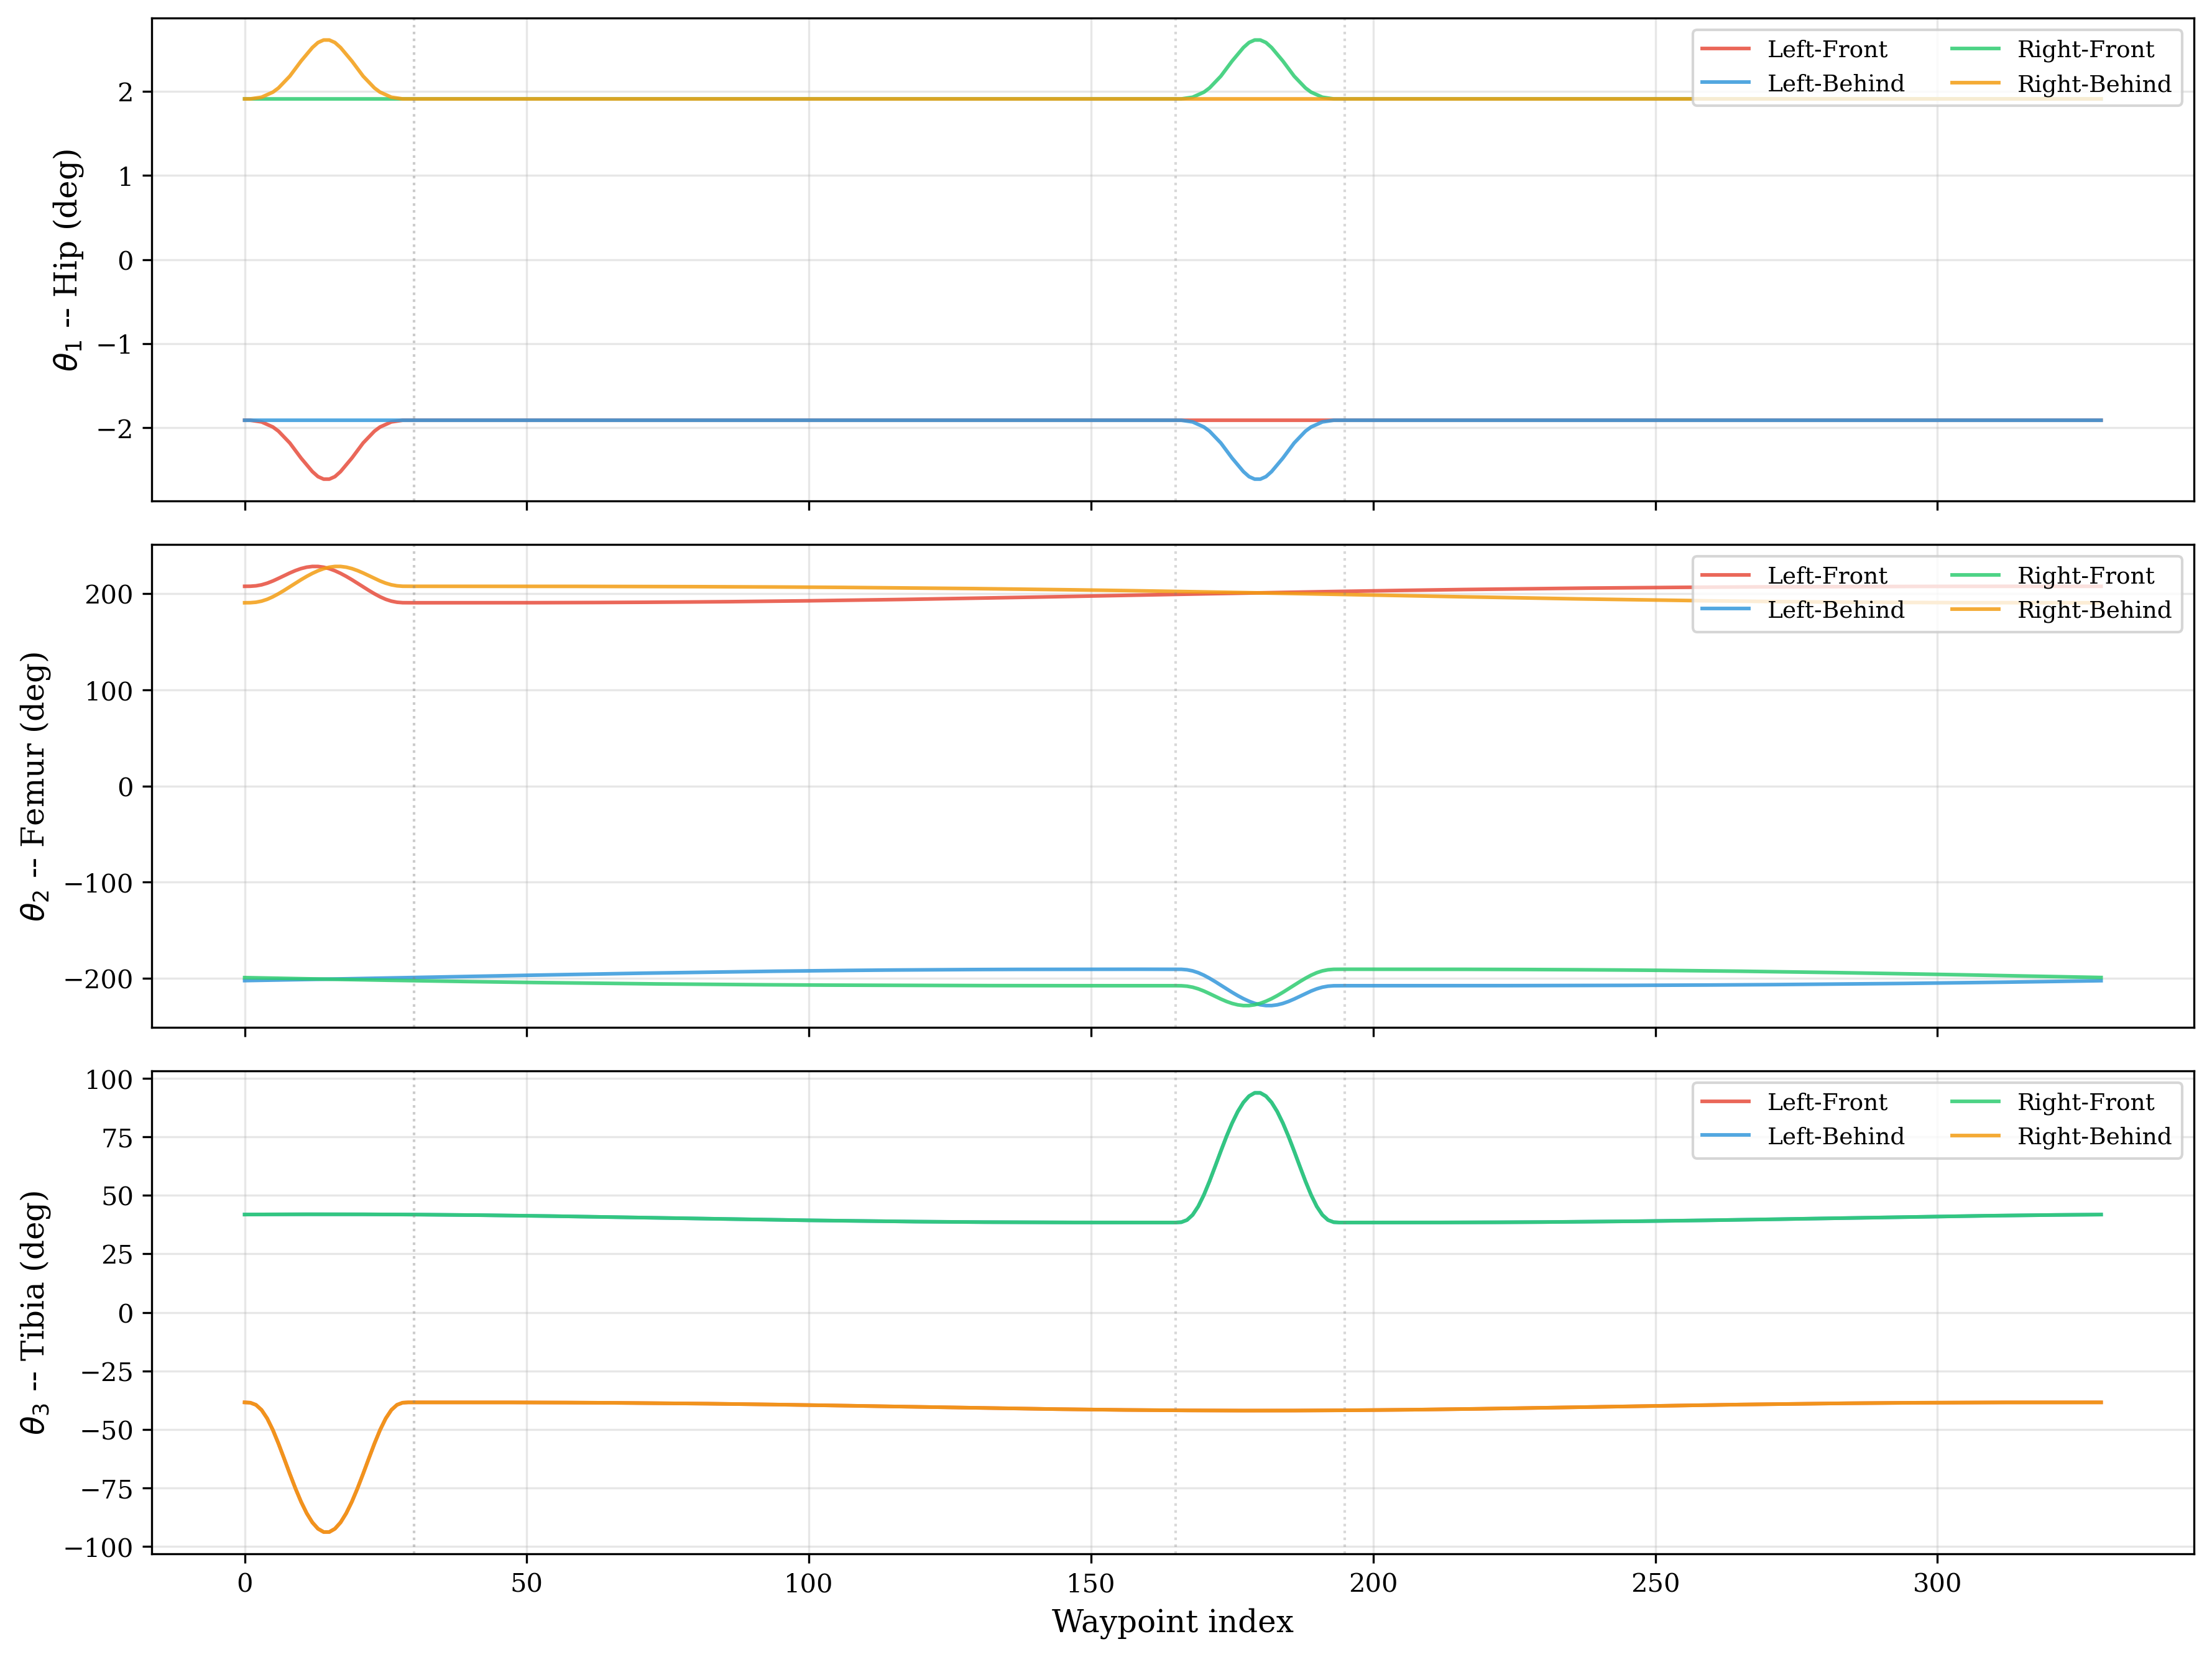
\includegraphics[width=0.6\textwidth]{Simulation/fig4_joint_angles.png}
    \caption{Biến thiên góc khớp}
    \label{Simulation/fig4}
\end{figure}
Hình \ref{Simulation/fig4} trình bày ba góc khớp đầu ra của thuật toán IK ($\theta_1$, $\theta_2$, $\theta_3$) theo đơn vị độ cho cả bốn chân trong một chu kỳ dáng đi đầy đủ gồm $T_{\text{total}} = 340$ waypoints ($T_{\text{swing}} = 30$, $T_{\text{stance}} = 310$).

Góc $\theta_1$ (khớp hip/coxa) điều khiển chuyển động abduction/adduction, dao động trong biên độ nhỏ ($\pm 2^\circ$) do robot di chuyển chủ yếu trong mặt phẳng sagittal. Hai chân bên trái có $\theta_1 < 0$, hai chân bên phải có $\theta_1 > 0$, phản ánh tính đối xứng cơ cấu.

Góc $\theta_2$ (khớp femur) có biên độ lớn nhất, liên quan trực tiếp đến chiều dài bước (stride length). Do cấu hình hình học ngược nhau giữa các cặp chân (left-front/right-behind và left-behind/right-front), $\theta_2$ có giá trị dương ($\sim 200^\circ$) cho một cặp và âm ($\sim -200^\circ$) cho cặp còn lại.

Góc $\theta_3$ (khớp tibia/gối) thay đổi rõ rệt trong pha swing khi bàn chân nâng lên để tránh va chạm mặt đất, với biên độ thay đổi khoảng $50^\circ$ so với vị trí stance. Hiệu ứng offset pha của dáng đi Trot được quan sát rõ: cặp LF+RB có pha swing tại waypoint 0–30, cặp LB+RF có pha swing tại waypoint 170–200 (lệch 50\% chu kỳ).

\subsection{Ước lượng mô-men xoắn bộ điều khiển PD}
\begin{figure}[H]
    \centering
    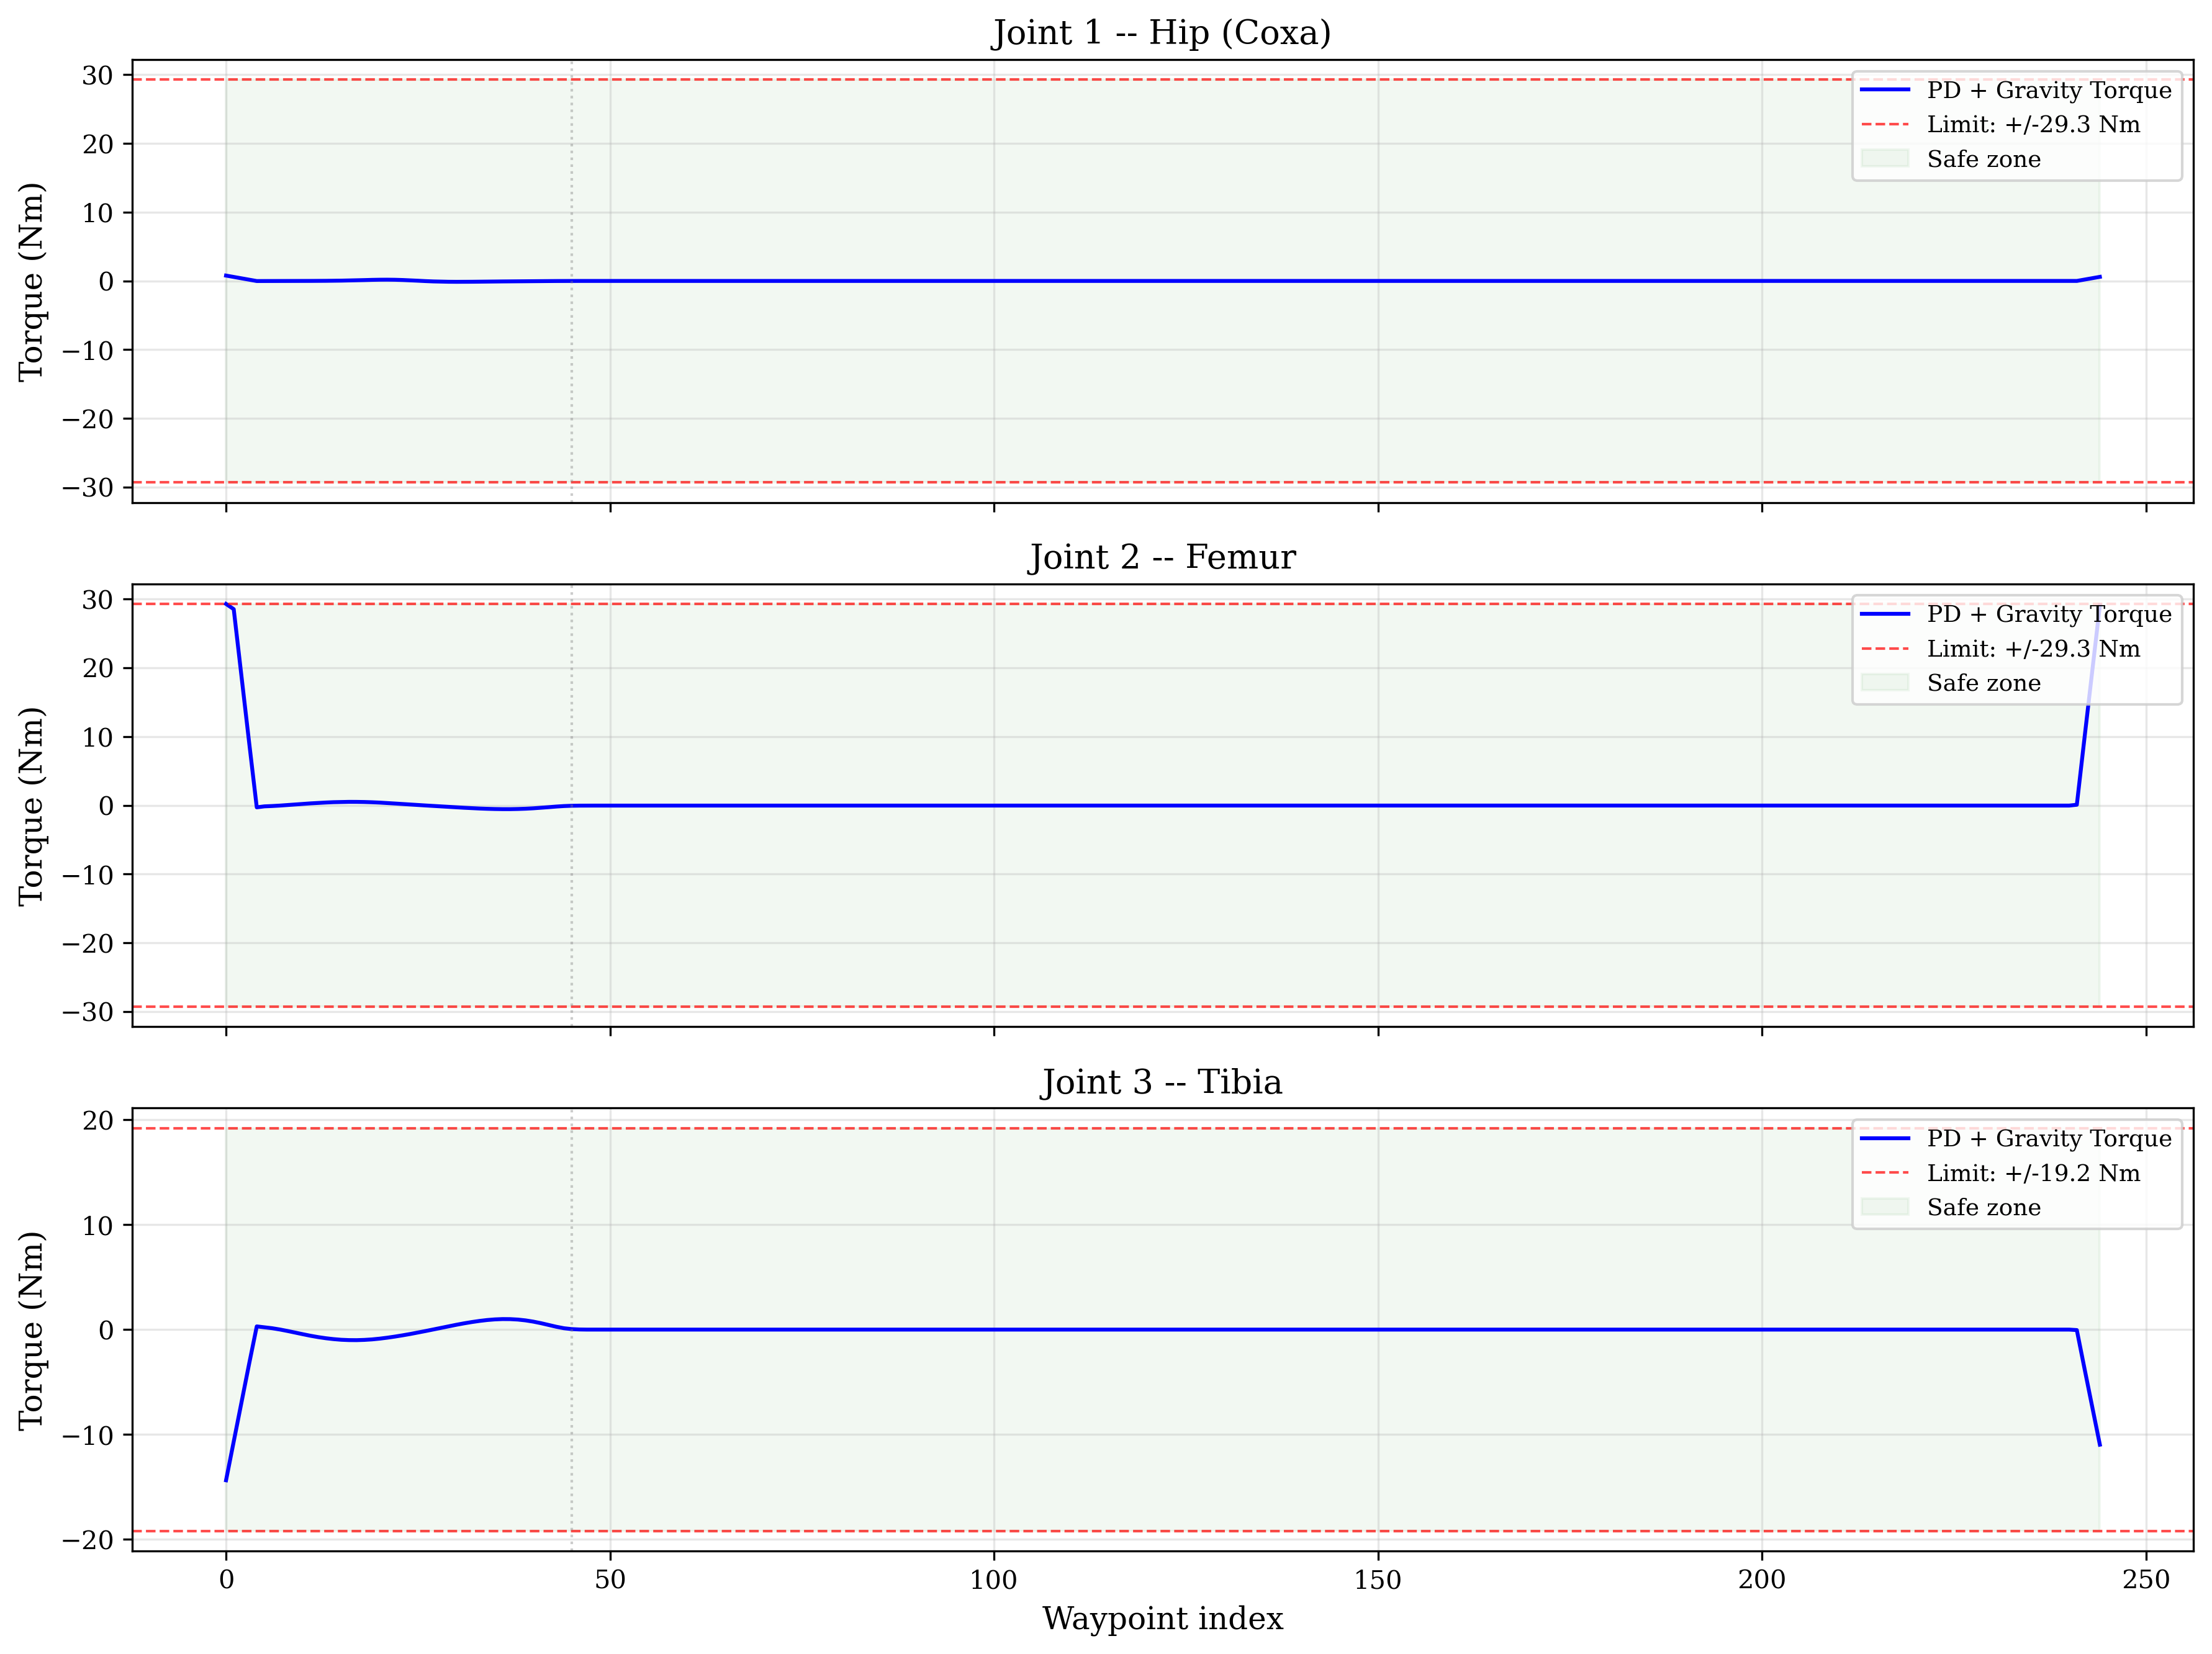
\includegraphics[width=0.6\textwidth]{Simulation/fig5_pd_torque.png}
    \caption{Mô-men xoắn bộ điều khiển PD}
    \label{Simulation/fig5}
\end{figure}
Hình \ref{Simulation/fig5} trình bày kết quả ước lượng mô-men xoắn cho chân Left-Front (chân tiêu biểu). Mô hình sử dụng luật điều khiển PD kết hợp bù trọng lực (gravity compensation):
\begin{equation}
    \tau_{\text{total}} = K_p \cdot (\theta_{\text{target}} - \theta_{\text{actual}}) - K_d \cdot \omega_{\text{actual}} + \tau_{\text{gravity}}
\end{equation}
trong đó $\tau_{\text{gravity}} = m \cdot g \cdot l_{\text{cg}} \cdot \cos(\theta)$ là mô-men trọng lực tại mỗi khớp, với $m$ là khối lượng link, $g = 9.81$ m/s$^2$ là gia tốc trọng trường, và $l_{\text{cg}}$ là khoảng cách đến trọng tâm link. Vị trí khớp thực tế ($\theta_{\text{actual}}$) được mô hình hóa như phiên bản lọc thông thấp (low-pass filter) của vị trí mong muốn, mô phỏng độ trễ bám theo (tracking delay) đặc trưng của servo.

Kết quả phân tích cho ba khớp:
\begin{itemize}
    \item \textbf{Khớp 1 (Hip):} Mô-men gần bằng $0$ Nm trong suốt chu kỳ do chuyển động abduction tối thiểu.
    \item \textbf{Khớp 2 (Femur):} Mô-men lớn nhất đạt khoảng $28$ Nm tại thời điểm bắt đầu pha swing, khi chân phải tăng tốc nhanh để nâng lên. Giá trị này nằm trong giới hạn effort của URDF ($\pm 29.3$ Nm), xác nhận servo đủ công suất.
    \item \textbf{Khớp 3 (Tibia):} Mô-men dao động trong khoảng $5\text{--}7$ Nm, nằm an toàn trong giới hạn ($\pm 19.2$ Nm).
\end{itemize}

Các đường gạch đỏ trên hình biểu thị giới hạn effort theo URDF, vùng tô xanh nhạt là vùng hoạt động an toàn (safe zone). Toàn bộ mô-men xoắn đều nằm trong vùng an toàn, xác nhận khả năng vận hành của bộ truyền động.

\section{Phân tích dáng đi và ổn định}

\subsection{Giản đồ thời gian dáng đi Trot}
\begin{figure}[H]
    \centering
    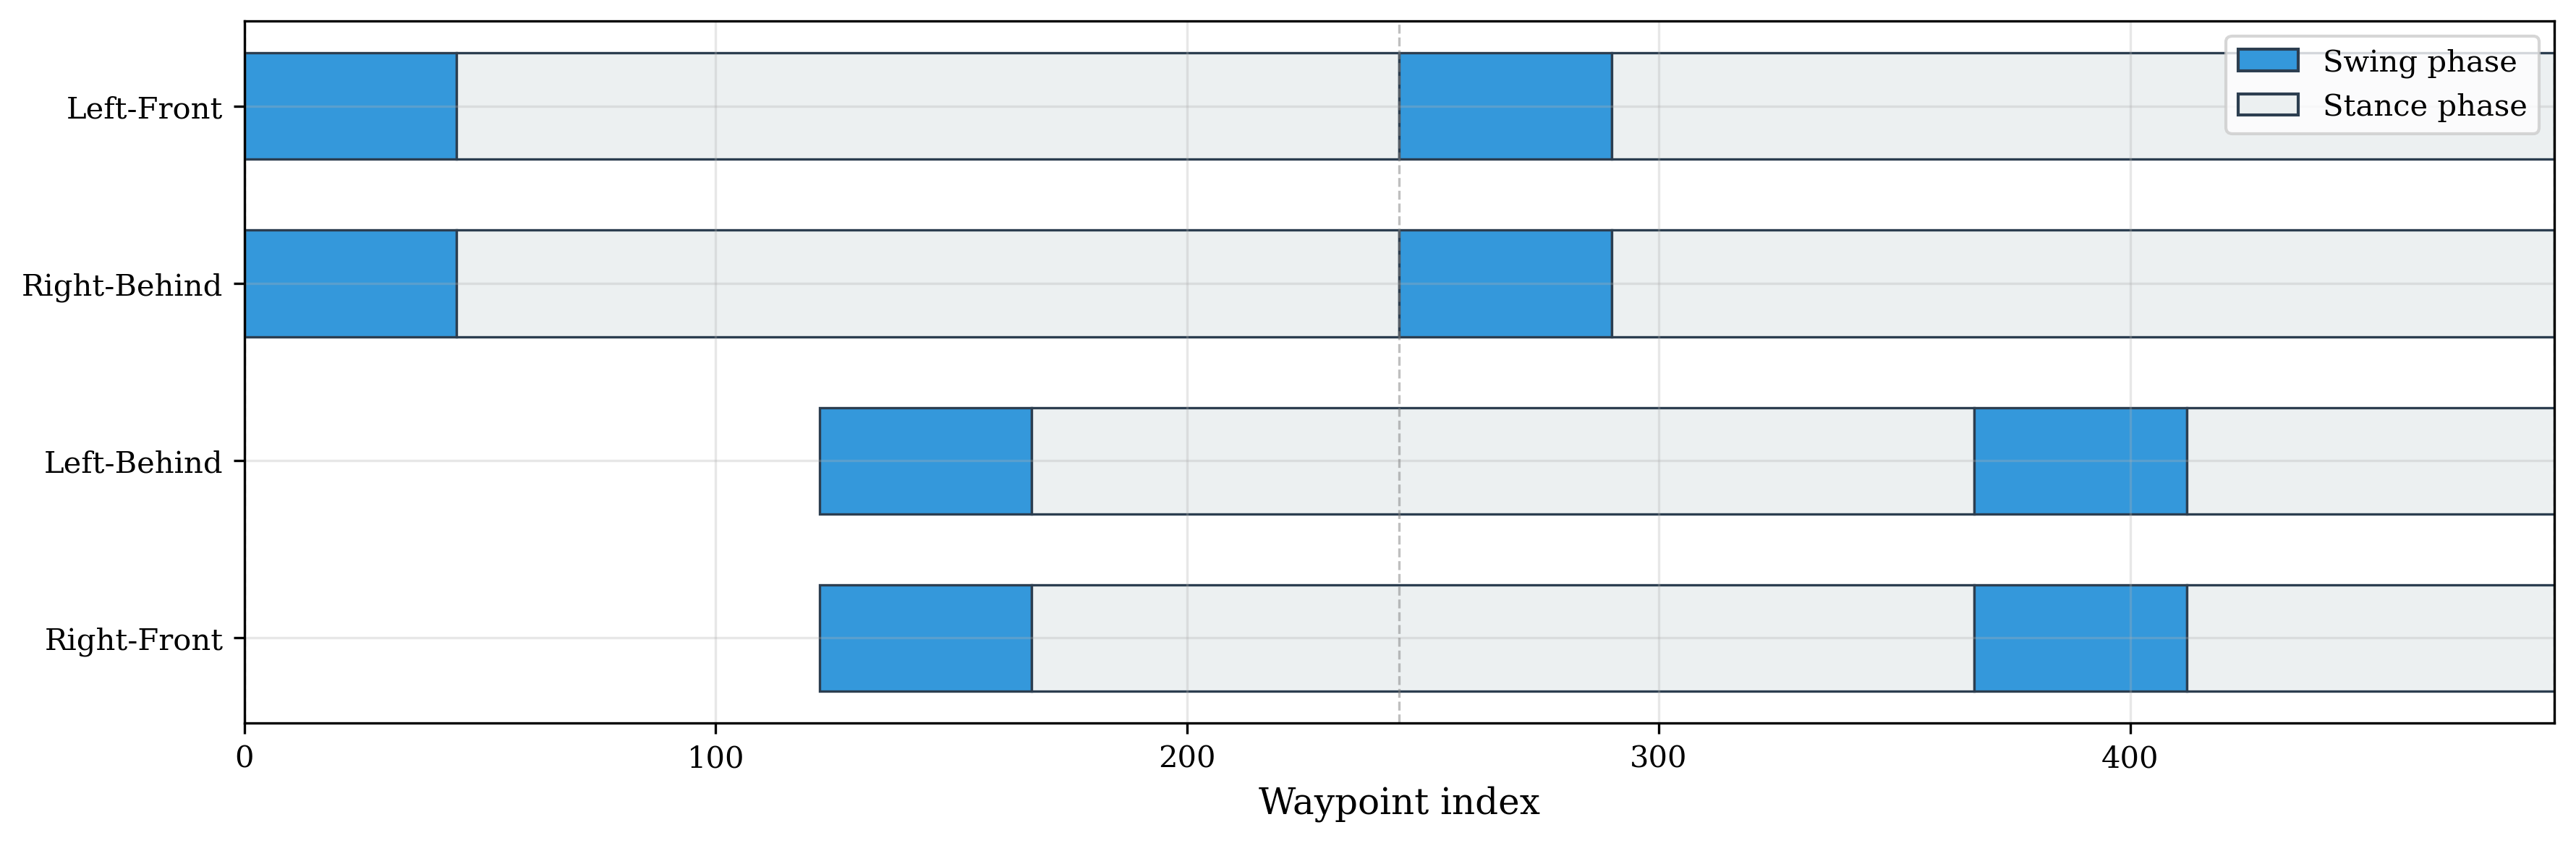
\includegraphics[width=0.6\textwidth]{Simulation/fig6_gait_timing.png}
    \caption{Gait timing}
    \label{Simulation/fig6}
\end{figure}
Hình \ref{Simulation/fig6} hiển thị giản đồ thời gian (timing diagram) của dáng đi Trot cho bốn chân, trong đó thanh màu xanh biểu thị pha swing và vùng trắng biểu thị pha stance.

Dáng đi Trot có hệ số chu kỳ nhiệm vụ $\beta = T_{\text{stance}} / T_{\text{total}} = 310/340 \approx 91{,}2\%$. Điều này có nghĩa mỗi chân ở trạng thái stance (chạm đất) khoảng 91,2\% thời gian và ở trạng thái swing (nâng chân) 8,8\% thời gian. Giá trị $\beta > 0{,}5$ đảm bảo tại mọi thời điểm luôn có ít nhất hai chân chạm đất. Hai cặp chân chéo nhau (LF+RB và LB+RF) luân phiên thực hiện pha swing với độ lệch pha 50\% chu kỳ.

\subsection{Đa giác đỡ và ổn định tĩnh}
\begin{figure}[H]
    \centering
    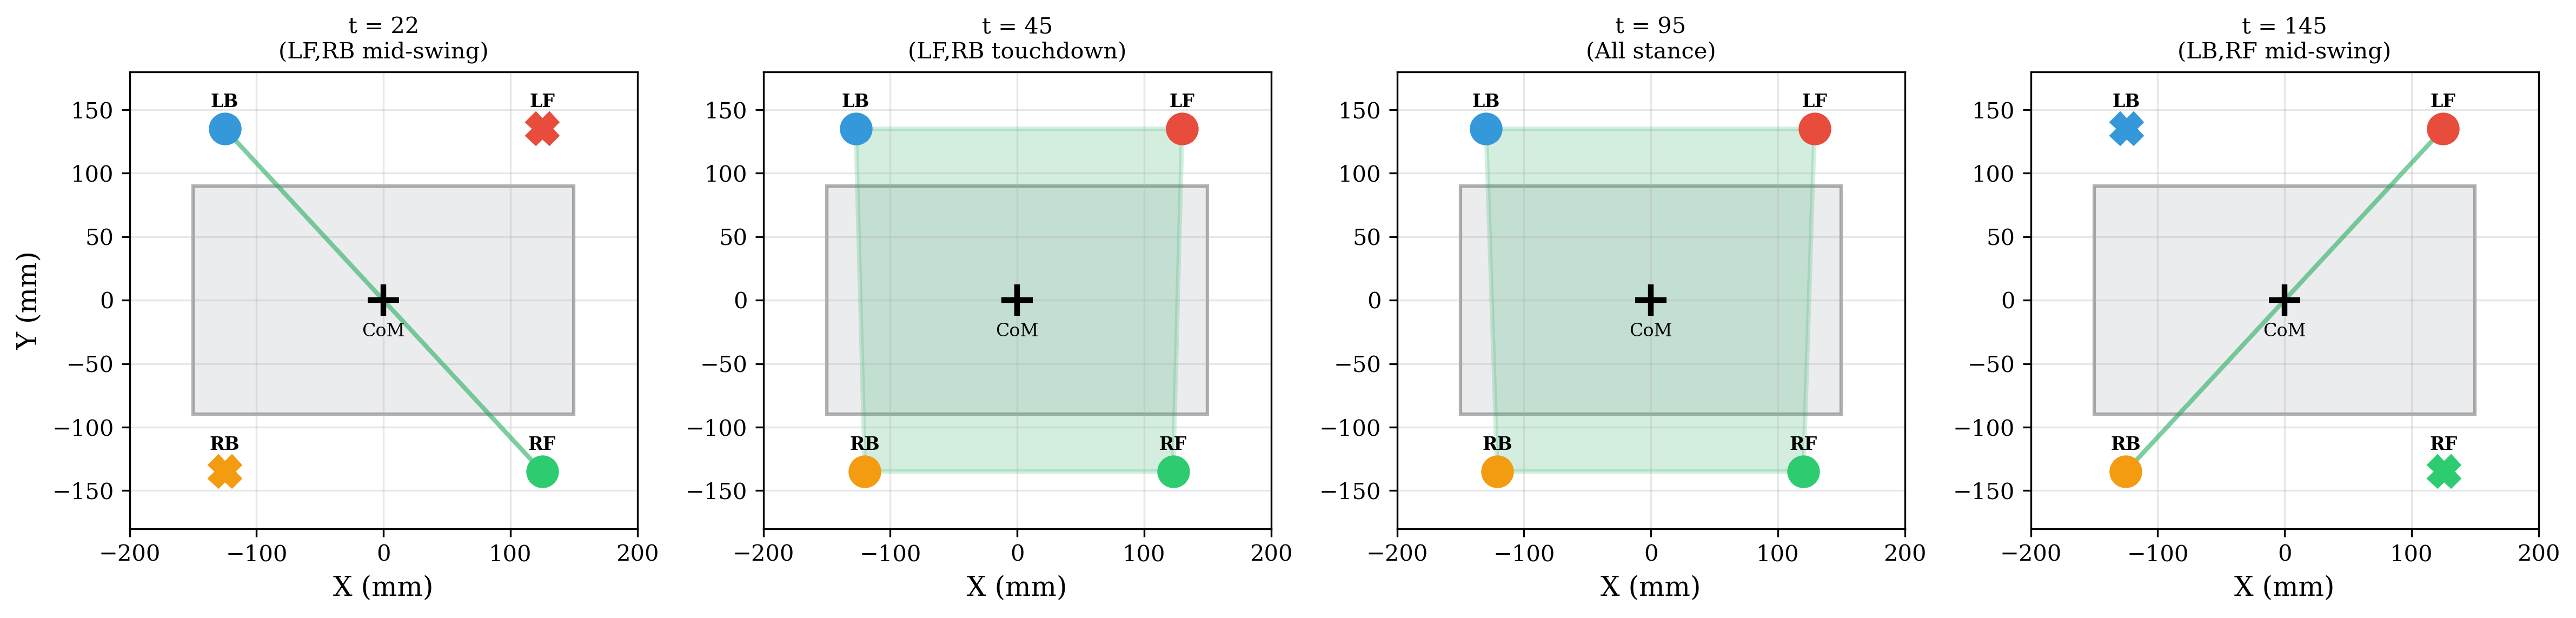
\includegraphics[width=0.6\textwidth]{Simulation/fig7_support_polygon.png}
    \caption{Đa giác đỡ và ổn định tĩnh}
    \label{Simulation/fig7}
\end{figure}
Hình \ref{Simulation/fig7} phân tích ổn định tĩnh bằng phương pháp đa giác đỡ (Support Polygon) tại hai thời điểm đặc trưng trong chu kỳ dáng đi.

Tại thời điểm $t = 0$ (pha swing của cặp LF+RB), chỉ có hai chân LB và RF chạm đất. Đa giác đỡ suy biến thành đoạn thẳng nối hai bàn chân. Hình chiếu trọng tâm (Center of Mass — CoM) của robot xuống mặt phẳng đỡ nằm gần đường thẳng này, cho thấy ổn định ở mức biên (marginal stability).

Tại thời điểm $t = T/4$ (pha stance đầy đủ), cả bốn chân đều chạm đất. Đa giác đỡ là hình chữ nhật bao quanh robot với diện tích lớn. Hình chiếu CoM nằm hoàn toàn bên trong đa giác đỡ, cho thấy ổn định tĩnh cao.

Tiêu chí ổn định được sử dụng: robot ổn định tĩnh khi và chỉ khi hình chiếu trọng tâm nằm trong bao lồi (convex hull) của các điểm tiếp xúc chân-đất. Kết quả xác nhận dáng đi Trot với các tham số đã chọn duy trì ổn định trong suốt chu kỳ.

\section{Không gian làm việc}
\begin{figure}[H]
    \centering
    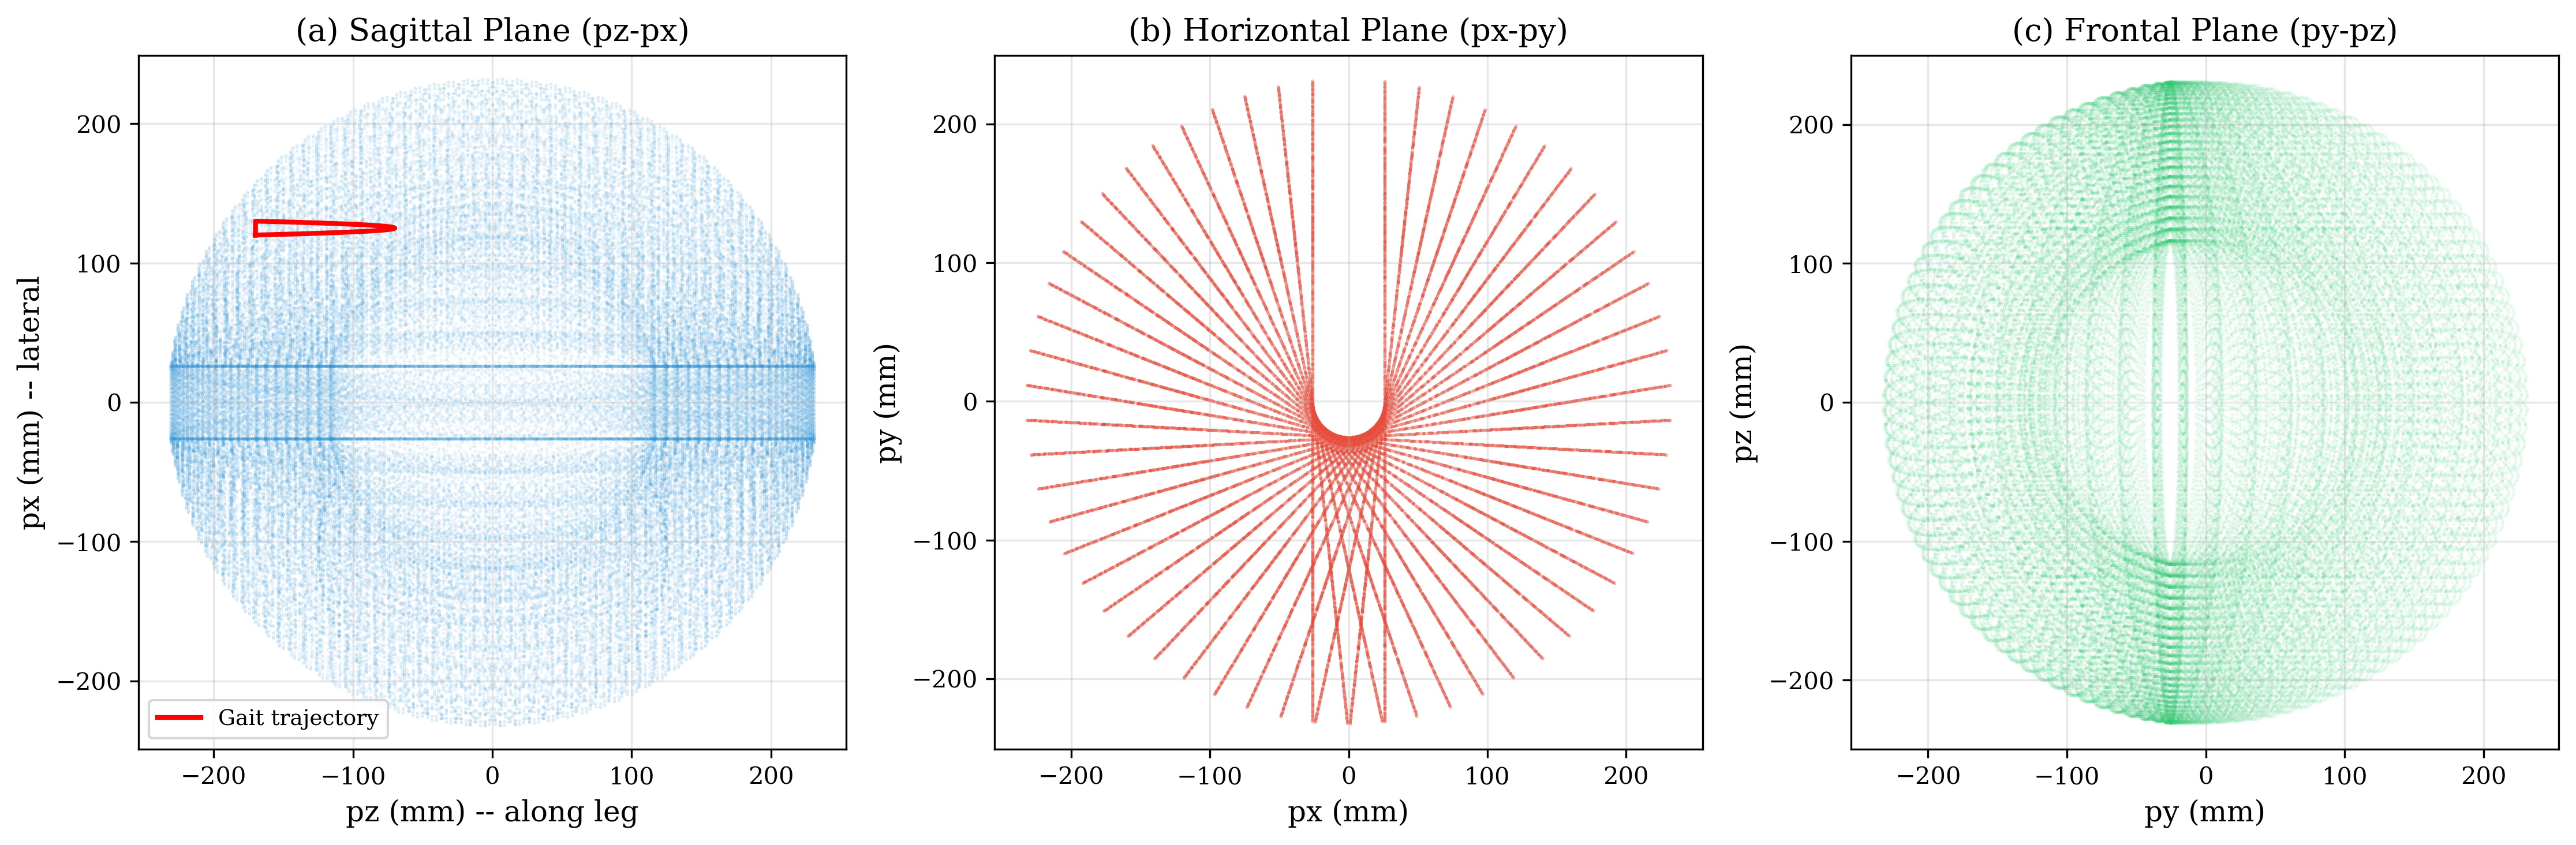
\includegraphics[width=0.6\textwidth]{Simulation/fig8_workspace.png}
    \caption{Không gian làm việc}
    \label{Simulation/fig8}
\end{figure}
Hình \ref{Simulation/fig8} trình bày không gian làm việc (workspace) của một chân robot 3-DOF, tính bằng phương pháp quét động học thuận (Forward Kinematics sweep).

Phương pháp tính toán bao gồm: quét toàn bộ miền góc khớp $\theta_1 \in [-30^\circ, 30^\circ]$, $\theta_2 \in [-90^\circ, 90^\circ]$, $\theta_3 \in [-90^\circ, 90^\circ]$ với khoảng 90.000 tổ hợp góc. Tại mỗi tổ hợp, tọa độ đầu chân trong hệ tọa độ chân (leg-local frame) được tính bằng phương trình FK và vẽ thành đám mây điểm 3D.

Kết quả cho thấy workspace có dạng \textbf{vòng cung} (annular sector), đặc trưng cho cơ cấu serial 3-DOF. Vùng đạt được rộng nhất trong mặt phẳng Y-Z (sagittal), trong khi chiều sâu theo phương X bị giới hạn bởi biên độ khớp hip ($\theta_1$). Tầm với tối đa của chân là $l_2 + l_3 = 80 + 80 = 160$ mm, tương ứng với trường hợp xương đùi và xương ống chân duỗi thẳng hoàn toàn.

\section{Tổng hợp tham số hệ thống}
Bảng \ref{tab:thamso_robot} tổng hợp các tham số chính của hệ thống mô phỏng.

\begin{table}[htbp]
\centering
\caption{Tham số hệ thống robot bốn chân}
\label{tab:thamso_robot}
\begin{tabular}{|l|c|c|l|}
\hline
\textbf{Tham số} & \textbf{Ký hiệu} & \textbf{Giá trị} & \textbf{Đơn vị} \\ \hline
Chiều dài thân robot & $L$ & 120 & mm \\ \hline
Chiều rộng thân robot & $W$ & 90 & mm \\ \hline
Chiều dài khớp coxa & $l_1$ & 20 & mm \\ \hline
Chiều dài xương đùi & $l_2$ & 80 & mm \\ \hline
Chiều dài xương ống chân & $l_3$ & 80 & mm \\ \hline
Hệ số tỷ lệ PD & $K_p$ & 20.0 & Nm/rad \\ \hline
Hệ số vi phân PD & $K_d$ & 0.5 & Nm$\cdot$s/rad \\ \hline
Giới hạn effort khớp hip & $\tau_{\max}$ (hip) & 29.3 & Nm \\ \hline
Giới hạn effort khớp tibia & $\tau_{\max}$ (tibia) & 19.2 & Nm \\ \hline
Số waypoint pha swing & $T_{\text{swing}}$ & 30 & waypoints \\ \hline
Số waypoint pha stance & $T_{\text{stance}}$ & 310 & waypoints \\ \hline
Độ cao nâng chân & $h$ & 40 & mm \\ \hline
Chu kỳ timer điều khiển & $T_{\text{timer}}$ & 3 & ms \\ \hline
Tốc độ cập nhật ros2\_control & $f_{\text{ctrl}}$ & 1000 & Hz \\ \hline
\end{tabular}
\end{table}

\section{Nhận xét và đánh giá}
Các kết quả mô phỏng cho phép rút ra một số nhận xét sau:

Thứ nhất, phương pháp lập kế hoạch quỹ đạo bằng đa thức bậc 5 cho kết quả vượt trội so với phương pháp sóng sin về mặt mượt mà động học. Biên dạng vận tốc và gia tốc liên tục (C$^2$) tại các điểm chuyển pha giúp giảm thiểu lực va đập và rung lắc tại các khớp, kéo dài tuổi thọ cơ cấu truyền động.

Thứ hai, bộ điều khiển PD với các tham số $K_p = 20{,}0$ Nm/rad và $K_d = 0{,}5$ Nm$\cdot$s/rad tạo ra mô-men xoắn nằm trong giới hạn cho phép của servo tại cả ba khớp. Mô-men lớn nhất xuất hiện tại khớp femur ($\sim 28$ Nm) vẫn thấp hơn giới hạn URDF ($29{,}3$ Nm), xác nhận bộ truyền động đủ công suất cho dáng đi Trot.

Thứ ba, dáng đi Trot với duty cycle $\beta \approx 91{,}2\%$ duy trì ổn định tĩnh trong suốt chu kỳ. Phân tích đa giác đỡ cho thấy biên ổn định nhỏ nhất xảy ra tại thời điểm chuyển pha khi chỉ có hai chân chạm đất, nhưng vẫn đảm bảo hình chiếu trọng tâm nằm trong vùng đỡ.

Thứ tư, không gian làm việc dạng vòng cung với tầm với tối đa 160 mm đủ lớn để thực hiện các bước đi trong phạm vi thiết kế. Kiến trúc phần mềm phân tầng (trajectory planning --- low-level control --- plant) cho phép mô phỏng trước khi triển khai trên phần cứng thực với thay đổi tối thiểu.

\section{Đánh giá hiệu năng bộ điều khiển PID nâng cao trên mô phỏng}

Phần này trình bày các kết quả thu được từ hệ thống mô phỏng, bao gồm dữ liệu chẩn đoán từ đường ống PID và các biên dạng quỹ đạo offline. Bảng~\ref{tab:pid_home_params} và Bảng~\ref{tab:pid_gait_params} tổng hợp toàn bộ tham số điều khiển cho hai chế độ hoạt động, được trích xuất trực tiếp từ mã nguồn hệ thống.

\begin{table}[H]
\centering
\caption{Tham số bộ điều khiển PID -- Chế độ tĩnh (HOME)}
\label{tab:pid_home_params}
\renewcommand{\arraystretch}{1.3}
\begin{tabular}{|l|c|c|l|}
\hline
\textbf{Tham số} & \textbf{Ký hiệu} & \textbf{Giá trị} & \textbf{Mô tả} \\ \hline
Hệ số tỷ lệ & $K_P$ & 2,0 & Khuếch đại sai lệch \\ \hline
Hệ số tích phân & $K_I$ & 0,30 & Triệt tiêu sai số xác lập \\ \hline
Hệ số vi phân & $K_D$ & 0,15 & Giảm chấn dao động \\ \hline
Bão hòa đầu ra & $u_{max}$ & 1,5 rad & Giới hạn tín hiệu hiệu chỉnh \\ \hline
Bão hòa tích phân & $\mathcal{I}_{max}$ & 1,5 & Chống windup \\ \hline
Rò rỉ tích phân & $\lambda$ & 0,9995 & Hệ số decay \\ \hline
Vùng chết đo & $d$ & 0,02 rad & Triệt nhiễu nhỏ \\ \hline
Ngưỡng gain schedule & $e_{thresh}$ & 0,08 rad & Ngưỡng tỷ lệ khuếch đại \\ \hline
Hệ số LPF đầu vào & $\alpha_{raw}$ & 0,4 & Lọc EMA tín hiệu thô \\ \hline
Hệ số LPF đạo hàm & $\alpha_d$ & 0,7 & Lọc thành phần D \\ \hline
Hệ số LPF đầu ra & $\alpha_c$ & 0,15 & Làm mượt tín hiệu bù \\ \hline
\end{tabular}
\end{table}

\begin{table}[H]
\centering
\caption{Tham số bộ điều khiển PID thích nghi -- Chế độ động (GAIT)}
\label{tab:pid_gait_params}
\renewcommand{\arraystretch}{1.3}
\begin{tabular}{|l|c|c|l|}
\hline
\textbf{Tham số} & \textbf{Ký hiệu} & \textbf{Giá trị} & \textbf{Mô tả} \\ \hline
Hệ số tỷ lệ & $K_P$ & 3,0 & Khuếch đại thích nghi \\ \hline
Hệ số tích phân & $K_I$ & 0,005 & Rất nhỏ (tránh dao động) \\ \hline
Hệ số vi phân & $K_D$ & 1,2 & Giảm chấn mạnh \\ \hline
Hệ số thích nghi P & $K_{prop}$ & 10,0 & Chia tỷ lệ adaptive gain \\ \hline
Vùng chết trung bình & $d_{avg}$ & 0,03 rad & Ngưỡng triệt nhiễu \\ \hline
Bão hòa đầu ra & $u_{max}$ & 0,30 rad & Giới hạn nhỏ hơn HOME \\ \hline
Bão hòa tích phân & $\mathcal{I}_{max}$ & 0,3 & Chống windup \\ \hline
Hệ số LPF đầu ra & $\alpha_{lpf}$ & 0,97 & Lọc mạnh hơn HOME \\ \hline
Số chu kỳ học baseline & $N_{learn}$ & 2 & Chu kỳ dáng đi \\ \hline
Tốc độ thích nghi baseline & $\eta_{adapt}$ & 0,05 & Cập nhật baseline \\ \hline
\end{tabular}
\end{table}

Sự khác biệt giữa hai bộ tham số phản ánh yêu cầu vận hành riêng biệt: chế độ HOME cần phản ứng nhanh ($K_P = 2{,}0$, $\alpha_c = 0{,}15$) để bù nhiễu loạn tức thời, trong khi chế độ GAIT cần lọc mạnh ($\alpha_{lpf} = 0{,}97$) và giới hạn đầu ra nhỏ ($u_{max} = 0{,}30$ rad) để tránh can thiệp quá mức vào quỹ đạo sải bước.

\subsection{Kết quả quy hoạch quỹ đạo offline}

Hình~\ref{fig_offline_traj_pos} trình bày quỹ đạo Cartesian $(x, y, z)$ của chân trước bên trái (Left-Front) trong một chu kỳ dáng đi đầy đủ gồm pha swing ($T_{swing} = 70$ frame) và pha stance ($T_{stance} = 200$ frame). Quỹ đạo trục $x$ thể hiện rõ chuyển động tiến/lùi với biên độ bước $L_{stride} = 45$ mm, trục $y$ duy trì ổn định, và trục $z$ cho thấy biên dạng nâng chân dạng parabol với độ cao $h_{lift} = 40$ mm.

\begin{figure}[H]
    \centering
    
\includegraphics[width=0.8\textwidth]{fig_offline_traj_pos.png}
    \caption{Quỹ đạo Cartesian $(x, y, z)$ của chân trước bên trái trong một chu kỳ dáng đi}
    \label{fig_offline_traj_pos}
\end{figure}

Hình~\ref{fig_offline_traj_vel_acc} trình bày biên dạng vận tốc và gia tốc tương ứng, xác nhận điều kiện biên $\dot{s}(0) = \dot{s}(1) = 0$ và $\ddot{s}(0) = \ddot{s}(1) = 0$ của hàm nội suy quintic.

\begin{figure}[H]
    \centering
    
\includegraphics[width=0.8\textwidth]{fig_offline_traj_vel_acc.png}
    \caption{Biên dạng vận tốc và gia tốc của chân trước bên trái}
    \label{fig_offline_traj_vel_acc}
\end{figure}

Hình~\ref{fig_offline_traj_angle} cho thấy các góc khớp $(\theta_1, \theta_2, \theta_3)$ đã giải qua IK, với pha swing và pha stance được tô màu phân biệt. Các chuyển tiếp góc khớp mượt mà, không có bước nhảy đột ngột, xác nhận tính đúng đắn của thuật toán IK.

\begin{figure}[H]
    \centering
    
\includegraphics[width=0.8\textwidth]{fig_offline_traj_angle.png}
    \caption{Góc khớp $(\theta_1, \theta_2, \theta_3)$ giải qua IK cho chân trước bên trái}
    \label{fig_offline_traj_angle}
\end{figure}

\subsection{Quỹ đạo 3D bàn chân trong môi trường mô phỏng}

Hình~\ref{fig_gait_3d_real} trình bày quỹ đạo 3D của chân trước bên trái trên hệ thống mô phỏng, cho thấy rõ hình dạng chữ D đặc trưng với cung swing phía trên và đường stance phẳng phía dưới.

\begin{figure}[H]
    \centering
    
\includegraphics[width=0.6\textwidth]{fig_gait_3d.png}
    \caption{Quỹ đạo 3D bàn chân chân trước bên trái trên hệ thống mô phỏng}
    \label{fig_gait_3d_real}
\end{figure}

\subsection{Ổn định tư thế tĩnh (chế độ HOME)}

Hình~\ref{fig_pid_home} trình bày đáp ứng sai lệch pitch và roll của bộ điều khiển PID trong chế độ HOME. Khi robot bị tác động nhiễu loạn bên ngoài (đẩy tay), sai lệch định hướng hội tụ nhanh chóng, ổn định hoàn toàn trong vùng chết $\pm 0{,}02$ rad trong khoảng $1{,}5$ giây sau nhiễu loạn. Kết quả này xác nhận cơ chế deadband và antiwindup hoạt động hiệu quả, tạo ra các lệnh servo có giảm chấn tới hạn phù hợp cho cân bằng tĩnh liên tục mà không gây dao động giới hạn quanh điểm đặt.

\begin{figure}[H]
    \centering
    
\includegraphics[width=0.85\textwidth]{fig_pid_error_home.png}
    \caption{Đáp ứng sai lệch bộ điều khiển trong chế độ tĩnh HOME}
    \label{fig_pid_home}
\end{figure}

\subsection{Ổn định động trong dáng đi Trot (chế độ GAIT)}

Hình~\ref{fig_pid_gait} trình bày sai lệch pitch và roll động trong pha dáng đi Trot. Mặc dù lực va chạm tuần hoàn từ mặt đất tạo ra các đỉnh sai lệch thoáng qua lên đến $\sim 0{,}15$ rad, các cơ chế thích nghi (moving average baseline, adaptive gain, zero crossing reset) trích xuất đúng xu hướng nghiêng bền vững từ các nhiễu tuần hoàn nghiêm trọng. Bộ điều khiển PID nhận biết pha giới hạn thành công sai lệch đỉnh trạng thái xác lập trong ngưỡng $0{,}08$ rad được định nghĩa bởi lịch trình hệ số khuếch đại, ngăn ngừa tích lũy trôi dài hạn và đảm bảo vận động phẳng liên tục ổn định.

\begin{figure}[H]
    \centering
    
\includegraphics[width=0.85\textwidth]{fig_pid_error_gait.png}
    \caption{Đáp ứng sai lệch bộ điều khiển trong chế độ động GAIT (dáng đi Trot)}
    \label{fig_pid_gait}
\end{figure}


%% ====================================================================
%%  PHẦN THỰC NGHIỆM PHẦN CỨNG
%% ====================================================================

\section{Thực nghiệm trên phần cứng thực}

\subsection{Giới thiệu}

Sau khi xác minh tính đúng đắn của các thuật toán thông qua mô phỏng ROS~2/Gazebo, toàn bộ hệ thống phần mềm được triển khai trên phần cứng thực nhằm đánh giá khả năng vận hành của robot trong điều kiện thực tế. Mục tiêu của giai đoạn thực nghiệm bao gồm:

\begin{itemize}
    \item Kiểm chứng khả năng homing (đưa robot về tư thế đứng) từ vị trí ngẫu nhiên.
    \item Đánh giá dáng đi Trot trên mặt phẳng nằm ngang.
    \item Kiểm tra cơ chế tắt an toàn (ROBOTOFF) ba pha.
    \item So sánh kết quả thực nghiệm với kết quả mô phỏng.
\end{itemize}

\subsection{Mô hình robot thực tế}

Mô hình robot bốn chân đã được lắp ráp hoàn chỉnh với các thành phần chính: khung thân in 3D (PLA), 12 động cơ bus servo ST3215, máy tính nhúng Jetson Nano B01, cảm biến IMU BNO055, hai mạch Bus Servo Adapter (A), mạch giảm áp XL4015 và nguồn xung tổ ong 12V--40A. Tổng khối lượng robot (không bao gồm nguồn và dây cáp) vào khoảng 2,3~kg.

\begin{table}[H]
\centering
\caption{Thông số hình học robot thực tế}
\label{tab:hw_robot_params}
\renewcommand{\arraystretch}{1.3}
\begin{tabular}{|l|c|c|l|}
\hline
\textbf{Tham số} & \textbf{Ký hiệu} & \textbf{Giá trị} & \textbf{Đơn vị} \\ \hline
Chiều dài thân robot & $L$ & 209 & mm \\ \hline
Chiều rộng thân robot & $W$ & 191 & mm \\ \hline
Chiều dài khớp coxa & $l_1$ & 26 & mm \\ \hline
Chiều dài xương đùi & $l_2$ & 106 & mm \\ \hline
Chiều dài xương ống chân & $l_3$ & 125 & mm \\ \hline
Tổng khối lượng robot & $m$ & $\sim$2,3 & kg \\ \hline
Số bậc tự do & DOF & 12 & -- \\ \hline
\end{tabular}
\end{table}

\subsection{Kiến trúc khởi động hệ thống phần cứng}

Hệ thống phần cứng thực được khởi động thông qua launch file ROS~2 chuyên dụng (\texttt{launch\_real.py}), bao gồm ba node chính:

\begin{itemize}
    \item \textbf{Serial Driver A} (\texttt{serial\_driver\_a}): Quản lý 6 servo thuộc chân trước bên trái (LF) và chân sau bên phải (RB), giao tiếp qua cổng \texttt{/dev/ttyACM1} với servo ID $[7, 8, 9, 10, 11, 12]$.
    \item \textbf{Serial Driver B} (\texttt{serial\_driver\_b}): Quản lý 6 servo thuộc chân sau bên trái (LB) và chân trước bên phải (RF), giao tiếp qua cổng \texttt{/dev/ttyACM0} với servo ID $[4, 5, 6, 1, 2, 3]$.
    \item \textbf{Leg Controller} (\texttt{node\_leg\_controller}): Tính toán động học nghịch, quy hoạch quỹ đạo và gửi lệnh điều khiển đến hai driver.
\end{itemize}

Mỗi serial driver nhận lệnh góc servo (đơn vị độ) từ topic \texttt{/servo\_commands\_a} hoặc \texttt{/servo\_commands\_b}, chuyển đổi sang giá trị tick (0--4095) và gửi qua giao tiếp UART bán song công đến các servo ST3215. Tốc độ truyền (baudrate) được cấu hình ở mức 1~Mbps để đảm bảo đáp ứng thời gian thực.

\subsection{Chuyển đổi góc IK sang góc servo}

Một thách thức quan trọng khi chuyển từ mô phỏng sang phần cứng thực là việc ánh xạ chính xác các góc khớp từ thuật toán IK sang giá trị điều khiển servo. Do cấu trúc lắp đặt cơ khí khác nhau giữa các chân (chiều quay ngược, offset vật lý), mỗi chân cần một hàm chuyển đổi riêng biệt. Các hàm này đã được hiệu chỉnh thực nghiệm (empirically verified) thông qua quá trình calibrate từng servo.

\begin{table}[H]
\centering
\caption{Công thức chuyển đổi IK → Servo cho từng chân}
\label{tab:ik_to_servo}
\renewcommand{\arraystretch}{1.5}
\begin{tabular}{|l|l|}
\hline
\textbf{Chân} & \textbf{Công thức chuyển đổi} \\ \hline
Left-Front (LF) & $s_1 = \theta_1 - 7$, \quad $s_2 = -(\theta_2 - 90) - 4$, \quad $s_3 = \theta_3 + 90$ \\ \hline
Left-Behind (LB) & $s_1 = \theta_1 + 5$, \quad $s_2 = \theta_2 + 356$, \quad $s_3 = \theta_3 + 90$ \\ \hline
Right-Front (RF) & $s_1 = \theta_1 + 7$, \quad $s_2 = -\theta_2 + 270$, \quad $s_3 = \theta_3 - 95$ \\ \hline
Right-Behind (RB) & $s_1 = \theta_1 + 5$, \quad $s_2 = -\theta_2 + 259$, \quad $s_3 = \theta_3 - 87$ \\ \hline
\end{tabular}
\end{table}

Trong đó $\theta_i$ là góc IK (độ) và $s_i$ là góc servo (độ). Giá trị servo sau đó được chuyển đổi sang tick bằng công thức: $\text{tick} = \text{offset} + \text{direction} \times s_i \times 4096 / 360$.

\subsection{Thử nghiệm Homing (chế độ ZERO)}

Quy trình homing đưa robot từ vị trí ngẫu nhiên ban đầu về tư thế đứng chuẩn. Hệ thống thực hiện các bước sau:

\begin{enumerate}
    \item \textbf{Đọc vị trí hiện tại:} Serial driver đọc vị trí feedback từ 12 servo qua giao thức phản hồi bán song công.
    \item \textbf{Tính toán tư thế đích:} Giải IK cho tư thế đứng chuẩn tại tọa độ bàn chân $(x, y, z)$ của từng chân, với bù trừ $z\_\text{offset}$ riêng cho mỗi chân để bù sai lệch cơ khí.
    \item \textbf{Nội suy tuyến tính:} Tạo quỹ đạo nội suy tuyến tính gồm 200 frame từ vị trí hiện tại đến vị trí đích cho cả 12 servo.
    \item \textbf{Vô hiệu hóa feedback:} Sau khi bắt đầu homing, feedback bị tắt trên cả hai driver để giải phóng đường truyền UART cho lệnh điều khiển.
    \item \textbf{Giữ tư thế:} Sau khi hoàn thành 200 frame, robot giữ tại vị trí đích.
\end{enumerate}

\begin{table}[H]
\centering
\caption{Tọa độ bàn chân tư thế đứng chuẩn và bù trừ chiều cao}
\label{tab:homing_targets}
\renewcommand{\arraystretch}{1.3}
\begin{tabular}{|l|c|c|c|c|}
\hline
\textbf{Chân} & $x$ (mm) & $y$ (mm) & $z_{\text{base}}$ (mm) & $z_{\text{offset}}$ (mm) \\ \hline
Left-Front (LF) & 125 & 135 & $-170$ & 0 \\ \hline
Left-Behind (LB) & $-125$ & 135 & $-170$ & $-5$ \\ \hline
Right-Front (RF) & 125 & $-135$ & $-170$ & $-1$ \\ \hline
Right-Behind (RB) & $-125$ & $-135$ & $-170$ & $-5$ \\ \hline
\end{tabular}
\end{table}

\subsection{Thử nghiệm dáng đi Trot (chế độ TROT\_FORWARD)}

Sau khi robot đạt tư thế đứng ổn định, dáng đi Trot được kích hoạt. Các tham số dáng đi trên phần cứng thực được trình bày trong Bảng~\ref{tab:hw_gait_params}.

\begin{table}[H]
\centering
\caption{Tham số dáng đi Trot trên phần cứng thực}
\label{tab:hw_gait_params}
\renewcommand{\arraystretch}{1.3}
\begin{tabular}{|l|c|c|l|}
\hline
\textbf{Tham số} & \textbf{Ký hiệu} & \textbf{Giá trị} & \textbf{Đơn vị} \\ \hline
Số waypoint pha swing & $T_{\text{swing}}$ & 45 & waypoints \\ \hline
Số waypoint pha stance & $T_{\text{stance}}$ & 200 & waypoints \\ \hline
Tổng waypoint/chu kỳ & $T_{\text{total}}$ & 245 & waypoints \\ \hline
Chiều dài bước & $L_{\text{stride}}$ & 10 & mm \\ \hline
Độ cao nâng chân & $h_{\text{lift}}$ & 100 & mm \\ \hline
Cao độ pha stance & $z_{\text{stance}}$ & $-170$ & mm \\ \hline
Phương pháp nội suy & -- & Đa thức bậc 5 & -- \\ \hline
Duty cycle & $\beta$ & 81,6\% & -- \\ \hline
\end{tabular}
\end{table}

Dáng đi Trot sử dụng mảng dịch pha: LF = 0,0; RB = 0,0; LB = 0,5; RF = 0,5, nghĩa là cặp chân chéo (LF+RB) và (LB+RF) luân phiên thực hiện pha swing. Quỹ đạo bàn chân được tạo bằng hàm nội suy đa thức bậc 5 (quintic planning) với điều khiển vận tốc, đảm bảo tính liên tục $C^2$.

\subsection{Cơ chế tắt an toàn (ROBOTOFF)}

Để đảm bảo an toàn khi dừng hoạt động, hệ thống triển khai quy trình tắt máy ba pha (three-phase shutdown) trực tiếp trong không gian góc servo, không sử dụng IK. Mỗi pha gồm 300 frame với chu kỳ $\sim$7~ms/frame, tổng thời gian tắt khoảng 6,3 giây.

\begin{table}[H]
\centering
\caption{Quy trình tắt an toàn ba pha (ROBOTOFF)}
\label{tab:robotoff}
\renewcommand{\arraystretch}{1.4}
\begin{tabular}{|c|p{0.15\linewidth}|p{0.45\linewidth}|c|}
\hline
\textbf{Pha} & \textbf{Khớp} & \textbf{Mô tả} & \textbf{Thời gian} \\ \hline
1 & Joint 3 (gối) & Gập gối → thân robot hạ xuống đất. LF/LB: $-47^\circ$, RF/RB: $+47^\circ$ & $\sim$2,1~s \\ \hline
2 & Joint 2 (vai) & Thu vai → chân gập sát thân robot. & $\sim$2,1~s \\ \hline
3 & Joint 1 (hông) & Xoè hông → chân xoè ra ngoài, robot nằm phẳng. & $\sim$2,1~s \\ \hline
\end{tabular}
\end{table}

Thiết kế tuần tự ba pha đảm bảo rằng robot không bao giờ rơi tự do: thân được hạ từ từ xuống đất trước khi các chân được thu gọn. Các giá trị góc đích có biên độ an toàn $\sim$3$^\circ$ so với giới hạn EEPROM của servo, tránh hiện tượng kẹt cơ khí.

\subsection{Các vấn đề thực tế và giải pháp}

Trong quá trình triển khai và thử nghiệm trên phần cứng thực, nhóm đã gặp và giải quyết một số vấn đề kỹ thuật quan trọng:

\begin{enumerate}
    \item \textbf{Sai lệch chiều cao giữa các chân:} Do dung sai gia công và lắp ráp, các chân robot có chiều cao không đồng đều khi đứng. Giải pháp: bổ sung tham số $z\_\text{offset}$ riêng cho từng chân (Bảng~\ref{tab:homing_targets}), được tinh chỉnh thủ công trong quá trình calibrate.

    \item \textbf{Chiều quay ngược giữa các chân:} Cấu trúc lắp đặt đối xứng gương khiến servo của chân trái và chân phải quay ngược chiều nhau cho cùng một chuyển động. Giải pháp: xây dựng hàm chuyển đổi IK-to-Servo riêng biệt cho từng chân với các hệ số offset và đổi dấu phù hợp.

    \item \textbf{Xung đột bus UART:} Khi cả lệnh điều khiển và phản hồi vị trí cùng chia sẻ một đường truyền UART bán song công, xảy ra hiện tượng xung đột dữ liệu. Giải pháp: vô hiệu hóa feedback sau khi hoàn tất bước đọc vị trí ban đầu trong quá trình homing.

    \item \textbf{Chia tải serial driver:} Một serial driver đơn lẻ không đủ băng thông để điều khiển đồng thời 12 servo ở tốc độ cao. Giải pháp: sử dụng hai serial driver (Driver A và Driver B), mỗi driver quản lý 6 servo thông qua một mạch Bus Servo Adapter riêng biệt.
\end{enumerate}

\subsection{Nhận xét và đánh giá thực nghiệm}

Kết quả thực nghiệm trên phần cứng cho phép rút ra các đánh giá sau:

Bảng~\ref{tab:sim_vs_hw} trình bày so sánh tổng quan giữa các tham số trong mô phỏng và trên phần cứng thực.

\begin{table}[H]
\centering
\caption{So sánh tham số giữa mô phỏng và phần cứng thực}
\label{tab:sim_vs_hw}
\renewcommand{\arraystretch}{1.3}
\begin{tabular}{|p{0.3\linewidth}|c|c|}
\hline
\textbf{Tham số} & \textbf{Mô phỏng} & \textbf{Phần cứng thực} \\ \hline
Kích thước thân ($L \times W$) & $120 \times 90$ mm & $209 \times 191$ mm \\ \hline
Chiều dài link ($l_1, l_2, l_3$) & 20, 80, 80 mm & 26, 106, 125 mm \\ \hline
Waypoint swing / stance & 30 / 310 & 45 / 200 \\ \hline
Duty cycle $\beta$ & 91,2\% & 81,6\% \\ \hline
Chiều dài bước & -- & 10 mm \\ \hline
Độ cao nâng chân & 40 mm & 100 mm \\ \hline
Bộ điều khiển & PD ($K_p=20$, $K_d=0,5$) & Servo PI nội bộ \\ \hline
Phản hồi IMU & Có (mô phỏng) & Có (BNO055 -- I2C) \\ \hline
\end{tabular}
\end{table}

\textbf{Thứ nhất}, quy trình homing hoạt động ổn định trên phần cứng thực. Robot được đưa từ vị trí ngẫu nhiên ban đầu về tư thế đứng chuẩn trong 200 frame ($\sim$1,4 giây với chu kỳ 7~ms/frame). Quá trình nội suy tuyến tính giữa vị trí feedback và vị trí đích IK tạo ra chuyển động mượt mà, không có hiện tượng giật hoặc va đập cơ khí.

\textbf{Thứ hai}, dáng đi Trot trên mặt phẳng nằm ngang cho thấy robot có khả năng di chuyển tiến liên tục. Tuy nhiên, do chiều dài bước ngắn ($L_{stride} = 10$ mm) và duty cycle cao ($\beta = 81{,}6\%$), tốc độ di chuyển tương đối chậm. Thiết kế này ưu tiên ổn định hơn tốc độ, phù hợp với giai đoạn kiểm chứng ban đầu.

\textbf{Thứ ba}, cơ chế tắt an toàn ba pha (ROBOTOFF) hoạt động đúng như thiết kế. Quy trình tuần tự gập gối → thu vai → xoè hông đảm bảo robot được hạ xuống đất an toàn trong mọi trường hợp. Tổng thời gian tắt khoảng 6,3 giây, đủ chậm để tránh lực quán tính gây hư hại cơ khí.

\textbf{Thứ tư}, việc chia hai serial driver (Driver A và Driver B) giải quyết hiệu quả vấn đề băng thông UART. Mỗi driver chỉ cần quản lý 6 servo, giảm tải truyền thông và đảm bảo thời gian đáp ứng dưới 7~ms cho toàn bộ 12 khớp.

\section{Phân tích sự khác biệt giữa mô phỏng và thực nghiệm}

Trong quá trình chuyển đổi từ mô phỏng sang phần cứng thực (sim-to-real transfer), nhóm đã nhận diện và ghi nhận một số khác biệt quan trọng:

\subsection{Khác biệt về kích thước mô hình}

Mô hình URDF sử dụng trong Gazebo có kích thước nhỏ hơn so với robot thực tế (Bảng~\ref{tab:sim_vs_hw}). Lý do chính là mô hình URDF được xây dựng trước trong giai đoạn thiết kế sơ bộ, trong khi robot thực tế có các điều chỉnh kích thước sau quá trình chế tạo và lắp ráp. Sự khác biệt này không ảnh hưởng đến tính đúng đắn của các thuật toán (FK, IK, PID) vì chúng được tham số hóa (parameterized), cho phép thay đổi kích thước link mà không cần sửa đổi mã nguồn.

\subsection{Khác biệt về tham số dáng đi}

Các tham số quỹ đạo trên phần cứng thực ($T_{swing} = 45$, $T_{stance} = 200$, $\Delta h = 100$ mm) khác biệt đáng kể so với mô phỏng ($T_{swing} = 30$, $T_{stance} = 310$, $\Delta h = 40$ mm). Lý do chính bao gồm:

\begin{itemize}
    \item \textbf{Độ cao nâng chân lớn hơn} (100 mm vs 40 mm): Do bề mặt thử nghiệm thực tế không hoàn toàn phẳng, robot cần nâng chân cao hơn để tránh va chạm khi bước. Trong mô phỏng Gazebo với mặt đất lý tưởng, 40 mm đã đủ.
    \item \textbf{Pha stance ngắn hơn} (200 vs 310 frame): Giảm thời gian pha stance giúp tăng tần số bước, cải thiện tốc độ di chuyển trên phần cứng thực.
    \item \textbf{Pha swing dài hơn} (45 vs 30 frame): Tăng thời gian pha swing giúp servo có đủ thời gian đáp ứng, do servo thực tế có độ trễ cơ khí mà mô phỏng không thể hiện hoàn toàn.
\end{itemize}

\subsection{Các yếu tố phi lý tưởng trên phần cứng thực}

Một số yếu tố phi lý tưởng (non-ideal factors) ảnh hưởng đến hiệu năng trên phần cứng thực mà mô phỏng không mô phỏng được:

\begin{itemize}
    \item \textbf{Ma sát và trượt bàn chân:} Vật liệu PLA của bàn chân có hệ số ma sát khác nhau trên các bề mặt thử nghiệm. Trên bề mặt trơn, robot có xu hướng trượt, giảm hiệu quả sải bước.
    \item \textbf{Độ dẻo cơ khí:} Các chi tiết in 3D (PLA) có độ dẻo nhất định, gây ra biến dạng nhỏ dưới tải trọng, dẫn đến sai lệch giữa vị trí bàn chân lý thuyết và thực tế.
    \item \textbf{Độ trễ truyền thông UART:} Giao thức UART bán song công giới hạn tốc độ cập nhật lệnh servo. Với baudrate 1~Mbps và 6 servo/driver, thời gian truyền một frame lệnh khoảng 1--2~ms, thấp hơn đáng kể so với chu kỳ điều khiển 7~ms.
    \item \textbf{Sai lệch lắp ráp:} Dung sai gia công và lắp ráp tạo ra sự không đồng đều về chiều cao giữa các chân, được bù bằng tham số $z\_\text{offset}$ riêng cho mỗi chân.
\end{itemize}